\section{Need for Defeaturing}\label{sec:defeaturing:need_defeaturing}

\todo{Review coomment: Move this (Section ...) here. [MOVED IT FURTHER IN PROPOSAL AS IT WAS NOT IN THE FLOW]}
\todo{Review comment: Here mention that which of the sheet metal features can be removed without affecting the gross shape. [THESE DETAILS ARE GIVEN A BIT LATER. THE DO NOT SEEM TO FEET AT THIS HIGH LEVEL ``NEED'' SECTION]}

\added{Literature survey Section~\ref{sec:survey:defeat} has reviewed various reported approaches of defeaturing. Subsection~\ref{sec:litsurvey:obsdefeat} concludes that these approaches did not adequately leverage the feature information and to a large extent did not consider application domain.}

The present research focuses on defeaturing \replaced{by leveraging feature information, of sheet metal features based CAD models. Lesser the features the model is built with, retaining the gross shape, easier the computation of midsurface}{for finding the gross shape needed in the computation of the ``Midsurface''}. Following experiment assesses this intuition, which has been formalized in the Hypothesis~\ref{hyp:Simplification} (Chapter~\ref{ch:Survey}).

%\subsection{Effect of defeaturing on the midsurface}
%		Many existing simplification methods recognize small, irrelevant features on a mesh or a solid body first, then remove them to get the simplified (called ``defeatured'')  model. Instead, if a Feature based CAD model is used as an input, then it has the advantage of the availability of ready features, so that the suppression and healing becomes relatively straightforward and robust. In such a feature based defeaturing method, the primary challenge is the identification of the suppressible features. In the past, the suppressibility used to be based on some insufficient criteria, like using full feature parameters, selecting all the negative features, etc. 

%Gross shape is the principal shape that ``represents'' the given shape but with far lesser features. Grossness depends on the size criteria, say, 5\% of the total volume/area. Features having sizes below this are the candidates for suppression.
%%\replaced{Lesser the part is covered with features, easier the computation of the midsurface. Sheet metal features like small Hole, Corner Round, Corner Chamfer, Hems, Rips, etc. can be removed, where as features like Wall, Flange, Bend, are retained.}{With lesser irrelevant details on the input model, the generated midsurface becomes more representative of the original part and the computation becomes robust (small deviations/features in the input do not affect the output in appreciable manner).} 


%%\bigskip

\begin{center}

\begin{tabular}[h]{@{} p{0.17\linewidth} |  p{0.25\linewidth} | p{0.25\linewidth} | p{0.22\linewidth}@{}} \toprule
\textbf{Part and \mbox{actions}} & \textbf{CAD Model} & \textbf{Generated \mbox{Midsurface}} & \textbf{Errors in \mbox{Midsurface}} \\ \midrule

Input model & 
\adjustbox{valign=t}{
 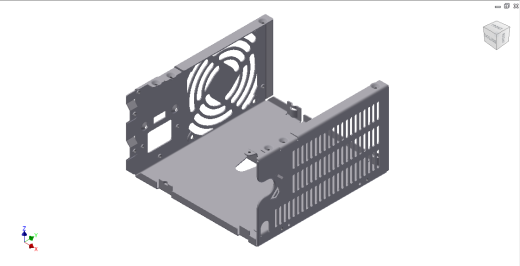
\includegraphics[width=\linewidth]{images/defeatmids_origpart} 
} &

\adjustbox{valign=t}{
 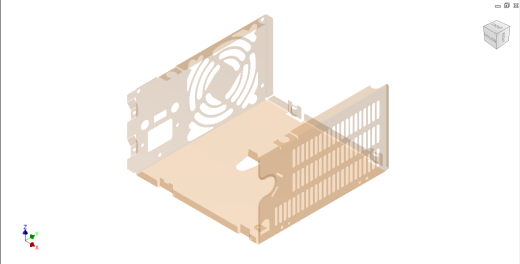
\includegraphics[width=\linewidth]{images/defeatmids_origmids} 
} &

Gaps and missing surfaces
\adjustbox{valign=t}{
 
\includegraphics[width=0.4\linewidth, angle=90]{images/defeatmids_origprobs} 
 } 

 \\

Defeaturing of the small irrelevant features. & 
\adjustbox{valign=t}{
 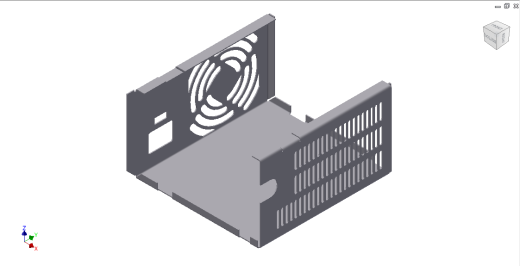
\includegraphics[width=\linewidth]{images/defeatmids_finpart} 
} &

\adjustbox{valign=t}{
 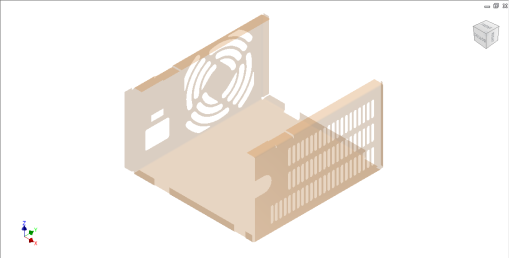
\includegraphics[width=\linewidth]{images/defeatmids_finmids} 
} &

No major errors. Good midsurface. \\

All negative features suppressed. & 
\adjustbox{valign=t}{
 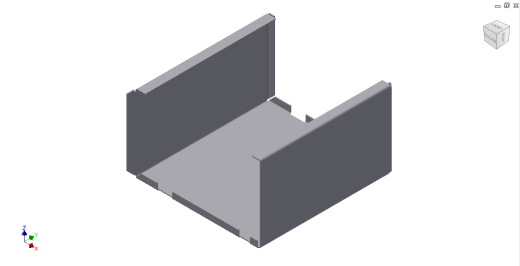
\includegraphics[width=\linewidth]{images/defeatmids_negpart} 
} &

\adjustbox{valign=t}{
 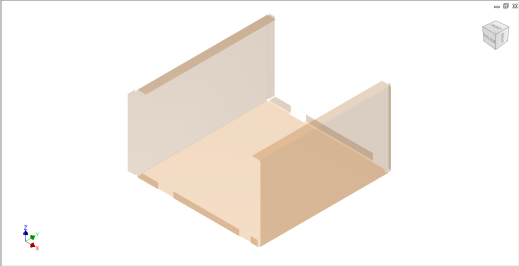
\includegraphics[width=\linewidth]{images/defeatmids_negmids} 
} &

No errors but midsurface lacks important shapes.\\

\bottomrule
\end{tabular}
\captionof{table}{Effect of Defeaturing on Midsurface Generation} \label{tbl:litsurvey:defeatmids}
\end{center}


%%\bigskip


\added{Table~\ref{tbl:litsurvey:defeatmids}  shows results of the experiment of studying the effect of defeaturing on the quality of the midsurface. The first row shows input CAD model and its midsurface computed using a commercial CAD-CAE system. The output midsurface shows various errors such as gaps and missing surfaces, as shown amplified in the picture under `Quality of Midsurface' column. The second row shows the effect of defeaturing, i.e. the removal irrelevant features, such as smaller holes, corner rounds, rips, hems, etc. It does not remove bigger holes, cutouts, flanges, grills, etc. The resultant midsurface does not show any major errors and is of good quality. The third row shows the effect of substantial defeaturing, i.e. removal of all the negative features, even if they are relevant. So all cutouts, patterns, grills, etc. are removed. The output midsurface, although has no gaps, or missing surfaces, lacks presence of the relevant negative features. Such defeaturing needs to be avoided as the midsurface does not represent the correct gross shape. Although this experiment validates the Hypothesis~\ref{hyp:Simplification} to be true, but suggests judicious selection of features for removal.}

\todo{Review comment: So how you have tackled the problem? write 2-3 lines on high level and mention that following section will provide details about the approach. [DONE]}

\added{The present research work, however, proposes use of the substantial defeaturing approach, i.e. the third row shown in Table~\ref{tbl:litsurvey:defeatmids}. Removal of  all the negative features simplifies the computation of midsurface to a large extent. The proposed approach overcomes the problem of missing relevant negative features on midsurface, by storing the tool bodies of those negative relevant features and bringing them back after computing the midsurface for piercing into it. With this arrangement, computing midsurface becomes easier and the output midsurface is not devoid of the impressions of relevant negative features.}

\added{Following section proposes a multi-phase approach for computing the `gross shape', which in turn, helps compute a quality midsurface.}

\section{Proposed Approach to Compute Gross Shape} \label{sec:defeaturing:overall_defeaturing}

\deleted{The concept of "gross shape" is subjective and hard to quantify~\cite{LeeLee1998}, but informal definition~\ref{def:grossshape} clarifies the expectation.} 

\todo{Review Comment: What is the purpose of this line? It doesn't reflect in the following. [REMOVED]}

%\begin{mydef}\label{def:grossshape}
%``gross shape'' is the shape arrived after defeaturing suppressible features, which retains the overall shape and characteristics. 
%\end{mydef}
In the context of the present research work, formulating rules for identification of the irrelevant features is the most critical step that affects the output gross shape.  \replaced{Researchers have measured the}{The} relevance of each feature by evaluation metrics~\cite{AdskElectronicsHelp}. 
%%Here is an example of rules for a particular domain, thermal analysis~\cite{AdskElectronicsHelp}: 
%%
%%	\begin{itemize} [noitemsep,topsep=2pt,parsep=2pt,partopsep=2pt]
%%	\item  Suppress all fasteners, related holes unless in critical heat path.
%%	\item  Suppress rip corners, bends and bend reliefs
%%	\item  Suppress gaps where tabs overlap.
%%%	\item  Replace perforation patterns with simple geometry
%%	\end{itemize}
%%

The evaluation metrics proposed in the present research is divided into three criteria, viz. application context-specific criteria, geometric reasoning-based criteria and dormant features criteria.

%%\bigskip

	\begin{figure} [!h]
		\centering
		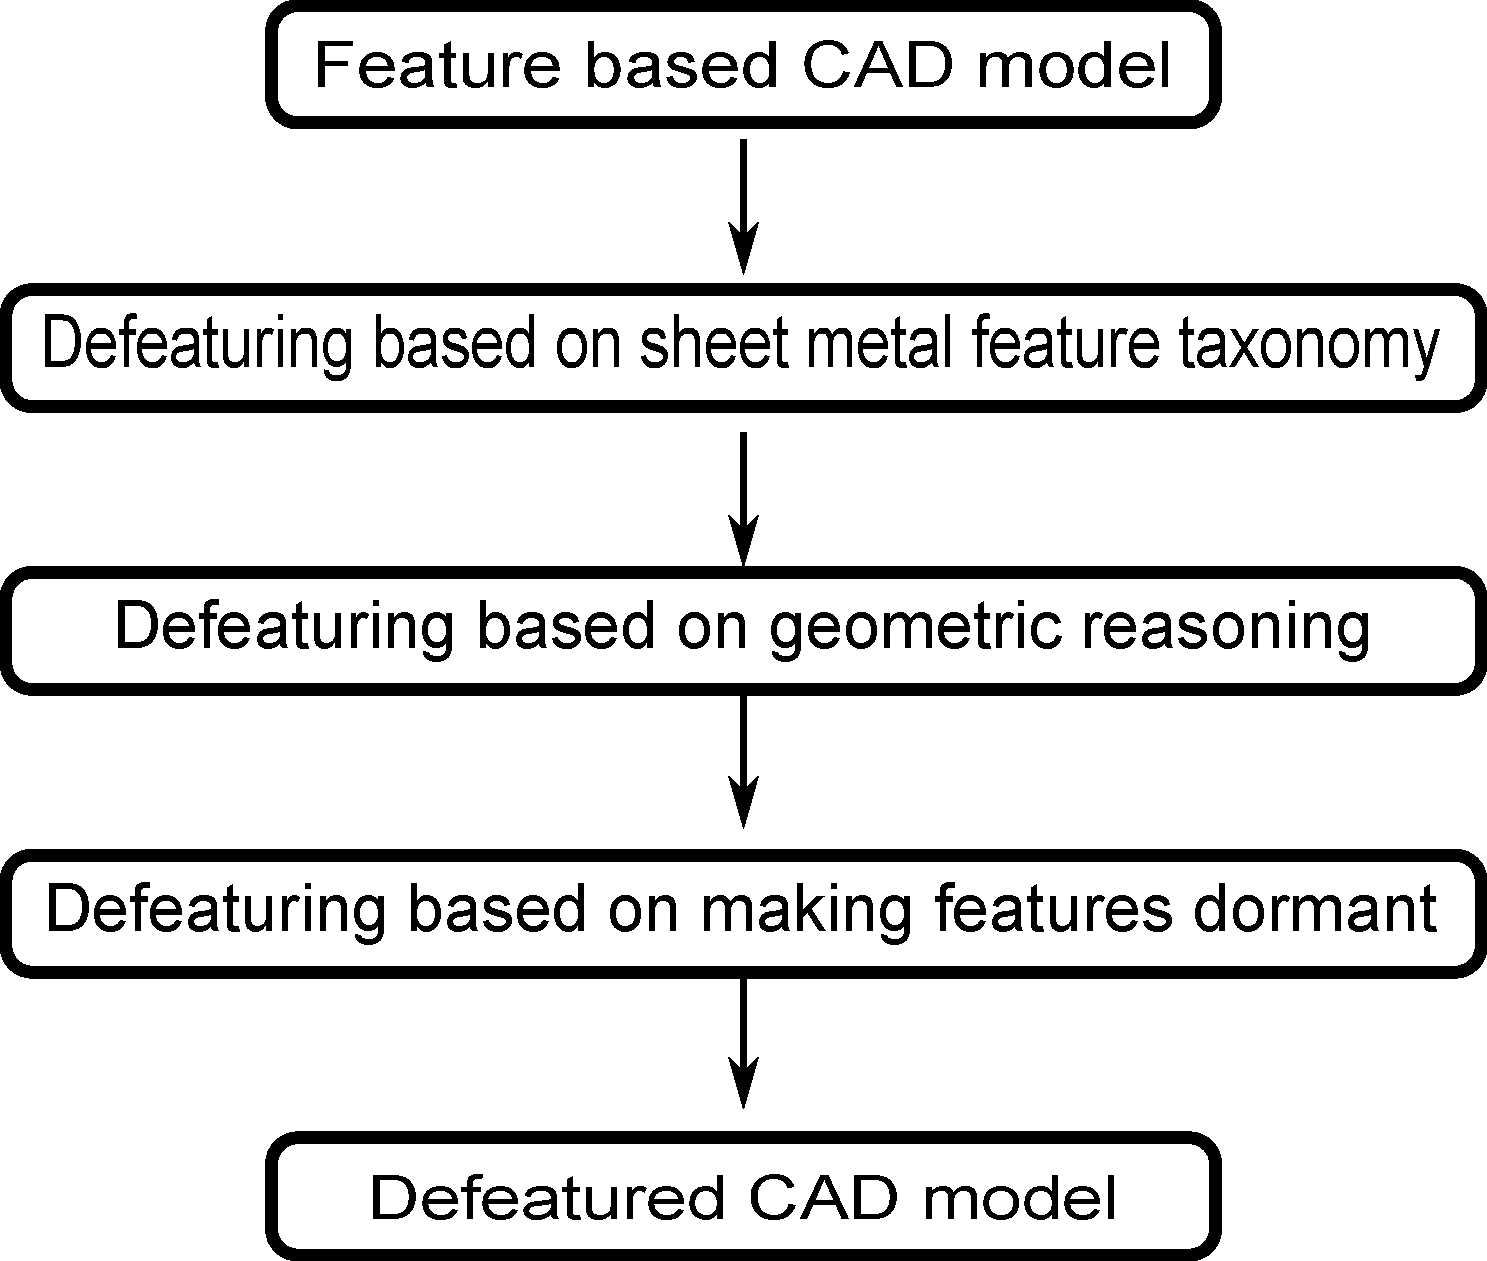
\includegraphics[width=0.5\linewidth]{images/SystemArchitectureDefeat_4.pdf}
		\caption{Overall Defeaturing Approach}
		\label{fig:defeaturing:OverallDefeaturingProcess}
	\end{figure}
	
%%\bigskip

 Figure~\ref{fig:defeaturing:OverallDefeaturingProcess} shows \added{phase-wise processing of the input sheet metal feature based CAD model by these criteria. Essentially these criteria apply various rules pertaining to application context, geometric reasoning and negative features, respectively. These rules are applied to identify the criticality of the features in the CAD model in the context of midsurface generation and attempts are made to remove not-so-relevant features from it. A threshold value is computed and provided to the overall approach. It denotes the ``size'' below which a feature is considered as irrelevant. The process thus simplifies the CAD model by defeaturing it while maintaining the gross shape intact. The phases of the proposed defeaturing process are explained below.}
	
\todo{Review comment: Directly start with the next section. [DONE]}
	
	\begin{itemize}
	[noitemsep,topsep=2pt,parsep=2pt,partopsep=2pt,leftmargin=*]
	\item \textbf{Phase I - Sheet Metal Taxonomy based}: The sheet metal CAD model feature tree is traversed and the candidate features for suppression are identified based on criteria based on the newly proposed sheet metal features taxonomy. For other domains or applications, this phase can be customized by employing application context specific taxonomies.
	
	\item \textbf{Phase II - Remnant Features}: This phase is generic and starts with the final Brep for identifying the remnant portions of the features. Those whose sizes are below the threshold are identified for suppression. One can customize the threshold based on engineering judgment appropriately.
	
	\item \textbf{Phase III - Dormant Bodies}: In this phase all ``negative'' features, even though they are relevant and thus have not been identified by the above two phases, are selected for removal, temporarily. Before removal, their feature bodies are cached/stored and are later used for re-applying on the output midsurface. 
	\end{itemize}
	

In the system implementing the proposed approach, it is important to note that, during defeaturing, even though the irrelevant features are said to be removed, they are discarded only temporarily and are not deleted permanently so that, in case of failure, they can be brought back and the original input CAD model to that stage can be restored.
 
%%%\begin{figure}[!ht]
%%%\RawFloats
%%\begin{minipage}[c]{0.95\linewidth}
%%    \begin{minipage}[c]{0.53\linewidth}
%%	\begin{itemize}
%%	[noitemsep,topsep=2pt,parsep=2pt,partopsep=2pt,leftmargin=*]
%%	\item \textbf{Phase I - Sheet Metal Taxonomy based}: The sheet metal CAD model feature tree is traversed and the candidate features for suppression are identified based on criteria based on the newly proposed sheet metal features taxonomy. For other domains or applications, this phase can be customized by employing application context specific taxonomies.
%%	
%%	\item \textbf{Phase II - Remnant Features}: This phase is gemeric and starts with the final Brep for identifying the remnant portions of the features. Those whose sizes are below the threshold are identified for suppression. One can customize the threshold based on engineering judgment appropriately.
%%	\end{itemize}
%%    \end{minipage}
%%    \hfill
%%    \begin{minipage}[c]{0.4\linewidth}
%%        \centering
%%        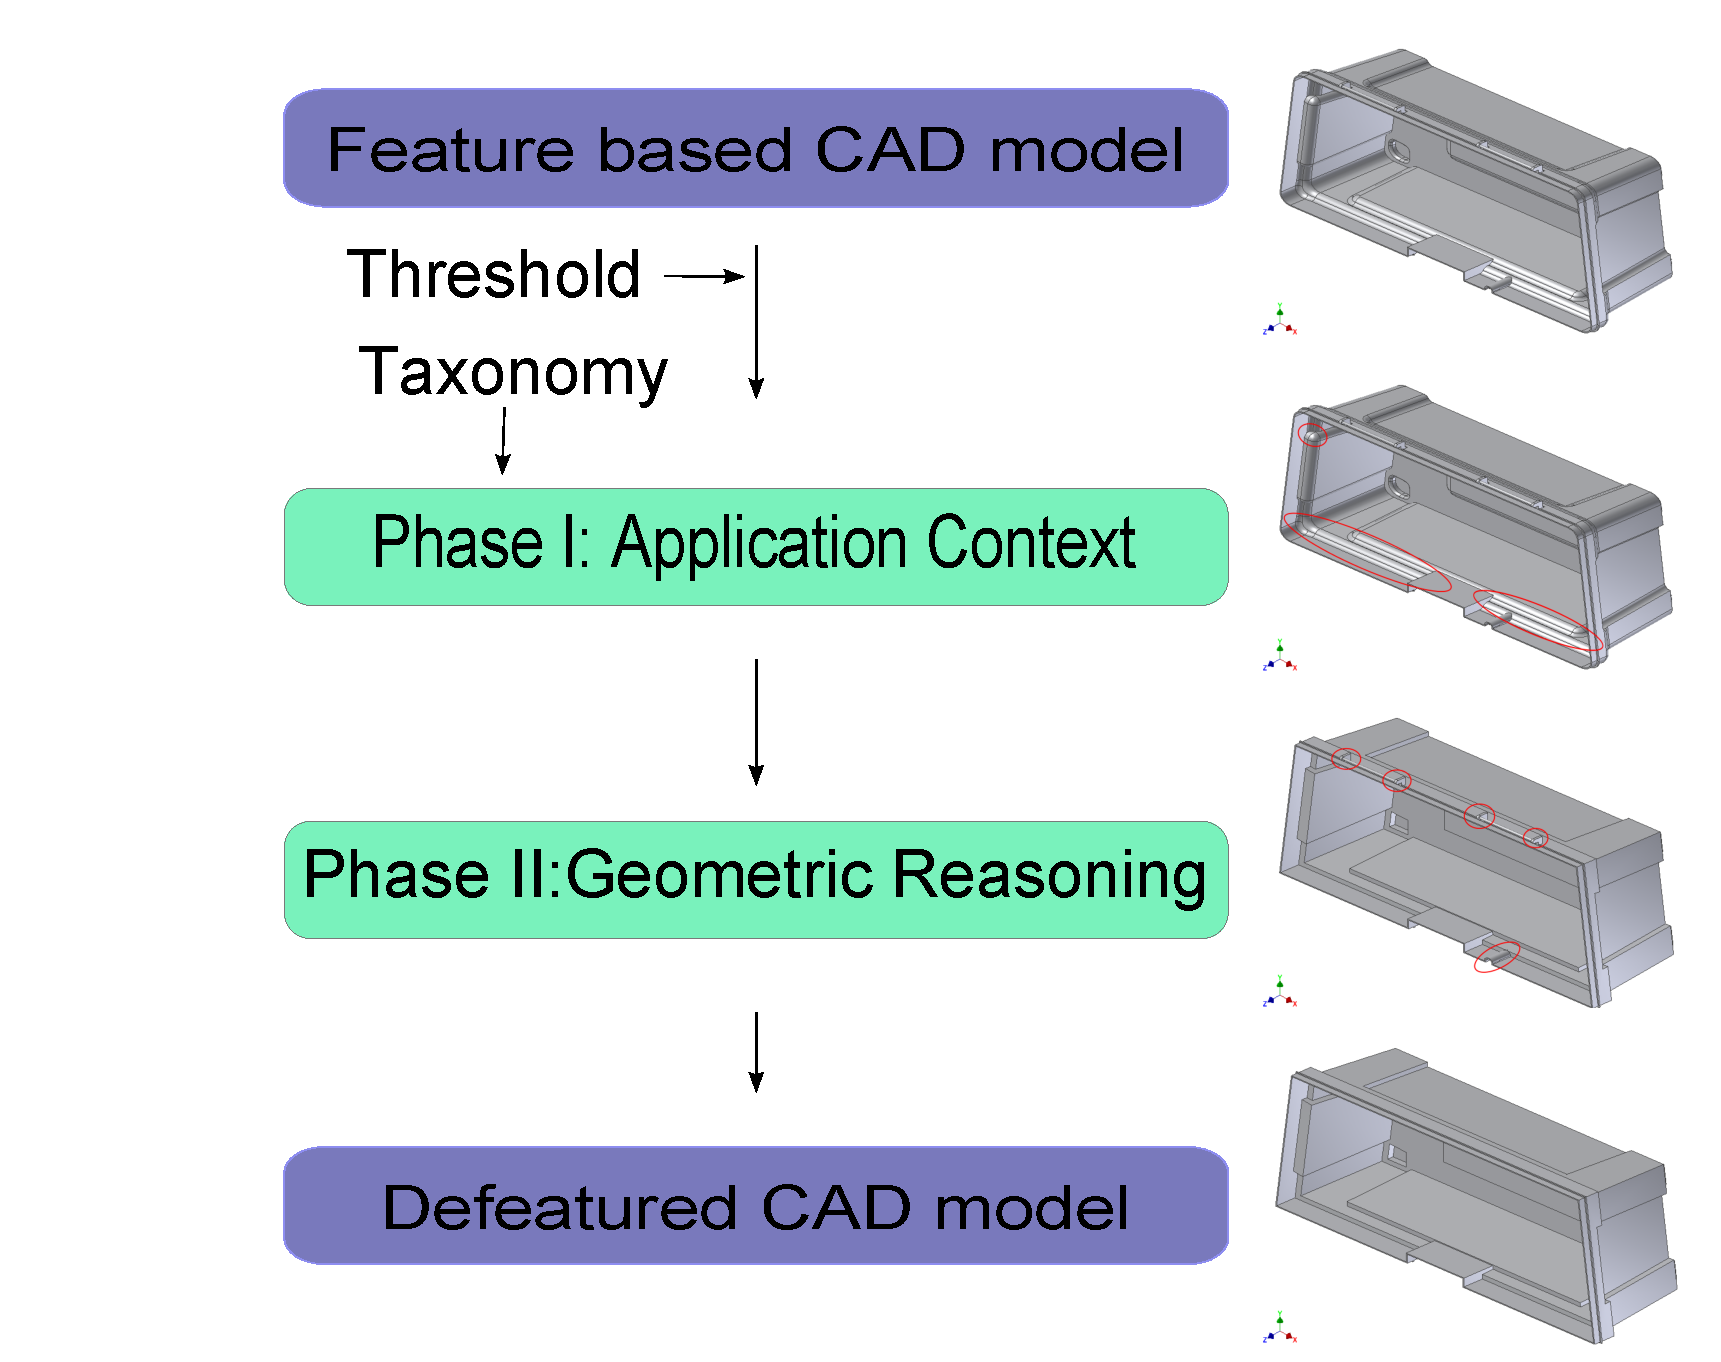
\includegraphics[width=\linewidth]{images/SystemArchitectureDefeat_1}
%%	 \captionof{figure}{Overall Process}
%%        	\label{fig:defeaturing:OverallDefeaturingProcess}           
%%    \end{minipage}
%%
%%\end{minipage}    
%%%\end{figure}

%The combined method (Phase I \& II) is called as ``\textbf{Smarf}'' (\textbf{S}heet \textbf{M}etal and \textbf{R}emnant \textbf{F}eatures). 
Following sections present the algorithms for these phases in details.


\section{Defeaturing Based on Sheet Metal Features \mbox{Taxonomy}}\label{sec:defeaturing:phase1}

CAD model under consideration is built by a number of sheet metal features such as Wall, Flange, Bend, etc. and are represented as a feature tree. This feature tree is traversed and the candidate features for removal are identified based on a criteria using the newly proposed sheet metal features taxonomy.

Figure ~\ref{fig:defeaturing:tax_sm} shows the proposed taxonomy which classifies sheet metal features and suggests their relevance with respect to maintaining the gross shape. In comparison with the other sheet metal features classifications, such as for features recognition~\cite{Gupta2013, Gupta2013a} and process planning~\cite{Kannan2009}, the proposed taxonomy is \replaced{different in a way that the classification is done based on the criticality of a particular feature to the gross shape.}{a novel one since the application context itself is different, and i.e. of finding the gross shape.}
%
%Sheet Metal parts are built using generic solid modeling features as well as some specialized sheet metal features. 
%
\subsection{Sheet Metal Features Taxonomy}\label{sec:defeaturing:phase11}

A thorough analysis of the inputs from various surveys with engineers and experts in the field to gauge relevance of sheet metal features with respect to the gross shape.  Proposed  taxonomy (Figure ~\ref{fig:defeaturing:tax_sm}) is the result of this analysis.

Taxonomy is represented by ``vocabulary'' and ``structure''~\cite{Tessier2011}. It is a scheme to represent and classify features for a particular purpose~\cite{Dartigues2005}.  Figure ~\ref{fig:defeaturing:tax_sm} shows the classification of sheet metal features for the purpose of computing gross shape.


%%\bigskip

%\begin{minipage}[c]{\linewidth}
\begin{center}
\begin{figure} [!h]
\dirtree{%
.1 Sheet Metal Features.
.2 Primary Features.
.3 Face-Wall   \adjustbox{valign=t}{
\includegraphics[scale=0.65]{images/InventorWall.png}}.
.3 Flange  \quad \adjustbox{valign=t}{
\includegraphics[scale=0.65]{images/InventorFlange.png}}.
.3 Bend   \qquad \adjustbox{valign=t}{
\includegraphics[scale=0.65]{images/InventorBend.png}}.
%.3 Loft Flange  \qquad \adjustbox{valign=t}{
\includegraphics[scale=0.65]{images/InventorLoftedFlange.png}}.
%.3 Rib \quad \quad  \adjustbox{valign=t}{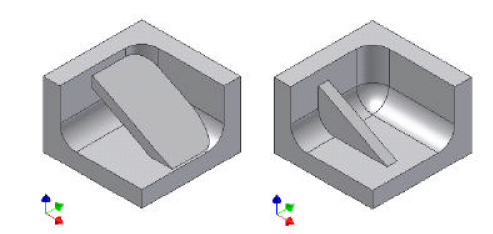
\includegraphics[height=0.11\linewidth]{images/Feature_Rib.png}}.
.2 Secondary Features.
.3 Stamping  \quad \adjustbox{valign=t}{
\includegraphics[scale=0.65]{images/InventorStamping.png}}.
.3 Cutout  \qquad \adjustbox{valign=t}{
\includegraphics[scale=0.65]{images/InventorCutout.png}}.
%.3 Fold  \qquad \adjustbox{valign=t}{
\includegraphics[scale=0.65]{images/InventorFold.png}}.
%.3 Roll  \qquad \adjustbox{valign=t}{
\includegraphics[scale=0.65]{images/InventorRoll.png}}.
.3 Emboss \qquad \adjustbox{valign=t}{
\includegraphics[scale=0.65]{images/InventorEmboss.png}}.
%.3 Hem   \quad \qquad \adjustbox{valign=t}{
\includegraphics[scale=0.65]{images/InventorHem.png}}.
%.3 Grill \qquad \adjustbox{valign=t}{
\includegraphics[scale=0.65]{images/InventorGrill.png}}.
.2 Tertiary Features.
%.3 Chamfer \qquad \adjustbox{valign=t}{
\includegraphics[scale=0.65]{images/InventorChamfer.png}}.
%.3 Round  \qquad \adjustbox{valign=t}{
\includegraphics[scale=0.65]{images/InventorRound.png}}.
%.3 Thread \qquad \adjustbox{valign=t}{
\includegraphics[scale=0.65]{images/InventorThread.png}}.
.3 Lip \qquad \adjustbox{valign=t}{
\includegraphics[scale=0.65]{images/InventorLip.png}}.
.3 Rest \qquad \adjustbox{valign=t}{
\includegraphics[scale=0.65]{images/InventorRest.png}}.
%.2 Connecting Features.
%.3 Bend   \qquad \adjustbox{valign=t}{
\includegraphics[scale=0.65]{images/InventorBend.png}}.
.2 Features Groups.
.3 Mirror \quad  \quad \adjustbox{valign=t}{
\includegraphics[scale=0.65]{images/InventorMirror.png}}.
%.3 RectPattern \quad  \adjustbox{valign=t}{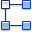
\includegraphics[scale=0.65]{images/InventorRectPattern.png}}.
.3 Pattern\quad  \adjustbox{valign=t}{
\includegraphics[scale=0.65]{images/InventorCircPattern.png}}.
}
\caption{Sheet Metal Features Taxonomy (Icons source: Autodesk Inventor~\cite{Inventor2014Help})}\label{fig:defeaturing:tax_sm}
\end{figure}
\end{center}

%%\bigskip

%\begin{tabular}[h]{@{} p{0.45\linewidth}  p{0.45\linewidth}@{}} 
%%\begin{minipage}[c]{0.98\linewidth}
%%\begin{minipage}[t]{0.5\linewidth}
\begin{itemize}
[noitemsep,topsep=2pt,parsep=2pt,partopsep=2pt, leftmargin=*]
\item \textbf{Primary Features}: These features mainly contribute to the gross shape. Examples are  Face-Wall, Flange, Bend, etc.
%	\begin{itemize} [noitemsep,topsep=2pt,parsep=2pt,partopsep=2pt]
%	\item Face-Wall
%	\item Flange
%	\item Bend
%	\end{itemize}
\item \textbf{Secondary Features}: Relevance of these features is based on the relative size with respect to the size of the whole model. Examples are Stamping, Cutout, Emboss, etc.
%	\begin{itemize} [noitemsep,topsep=2pt,parsep=2pt,partopsep=2pt]
%	\item Stamping
%	\item Cutout
%	\item Emboss 
%	\end{itemize}
	
\item \textbf{Tertiary Features}: These features are irrelevant to the gross shape irrespective of their size relative to the size of the whole model. Examples are Lip, Rest, etc.
%	\begin{itemize} [noitemsep,topsep=2pt,parsep=2pt,partopsep=2pt]
%	\item Lip
%	\item Rest 
%	\end{itemize}
	
%\item \textbf{Connecting Features}: These are not suppressed irrespective of their sizes, as removing them, will create gaps between the sub-shapes of the original part. Lacking these would create gaps, so these are retained irrespective of their relative size, small or large.
%Example is:
%	\begin{itemize} [noitemsep,topsep=2pt,parsep=2pt,partopsep=2pt]
%	\item Bend
%	\end{itemize}
		
\item \textbf{Feature Groups}: These are feature collections. Their relevance is assessed as a collection, similar to the secondary features. Examples are Mirror, Patterns, etc.
%\begin{itemize} [noitemsep,topsep=2pt,parsep=2pt,partopsep=2pt]
%	\item Mirror
%	\item Patterns
%	\end{itemize}
\end{itemize}


		
%
%\begin{minipage}[t]{0.4\linewidth}
%		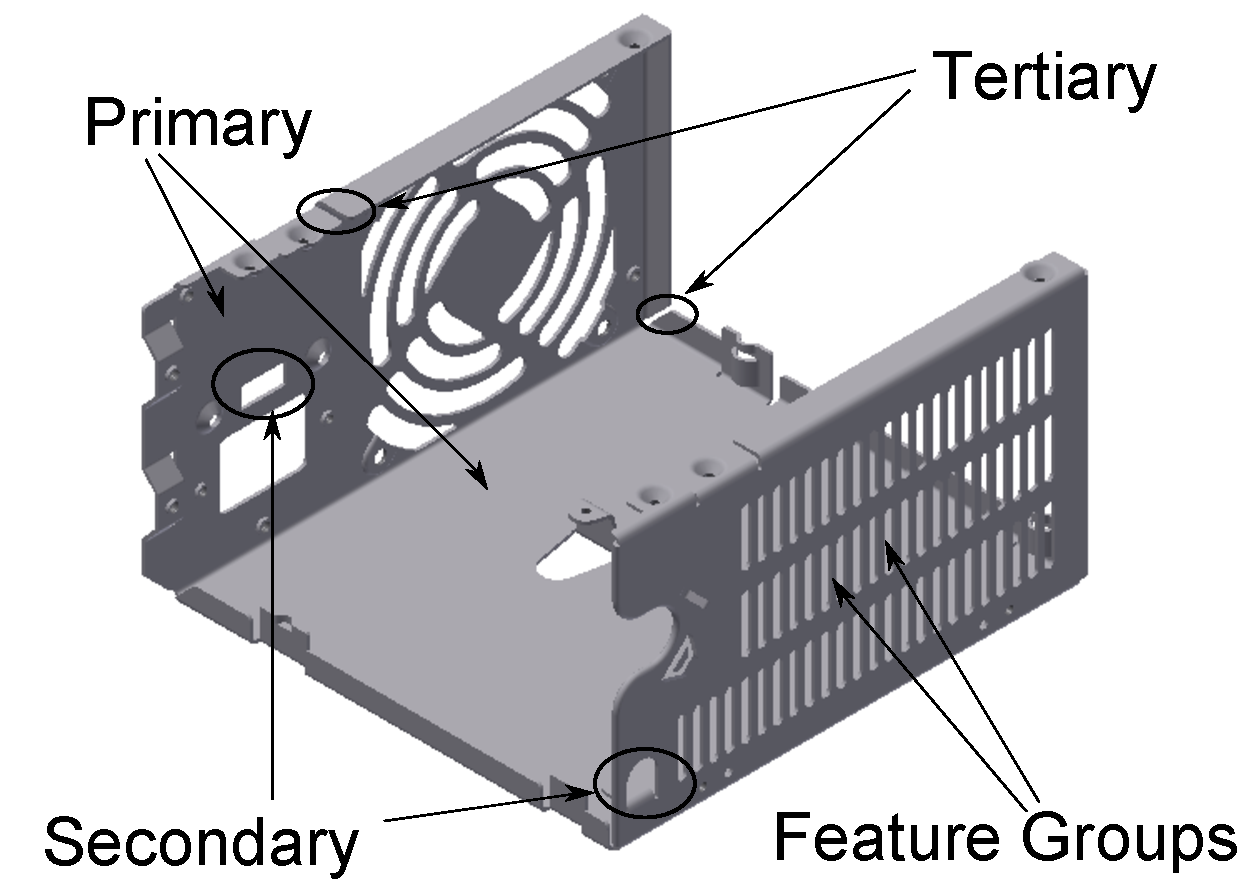
\includegraphics[width=\linewidth]{images/SheetMetal_taxonomy_2.pdf}
%		\captionof{figure}{Examples of classified types}
%		\label{fig:defeaturing:classification}
%\end{minipage}
%\end{minipage}    


Figure~\ref{fig:defeaturing:tax_sm} shows the proposed taxonomy classifying sheet metal features into categories such as Primary features, Secondary features, Tertiary features and Feature groups, based on their sheet metal domain specific characteristics. For defeaturing, each feature category undergoes its own rule for eligibility for removal during defeaturing process. Those rules are elaborated in detail in Section~\ref{sec:defeaturing:taxonomy}.

%%\bigskip

	\begin{figure} [!h]
		\centering
		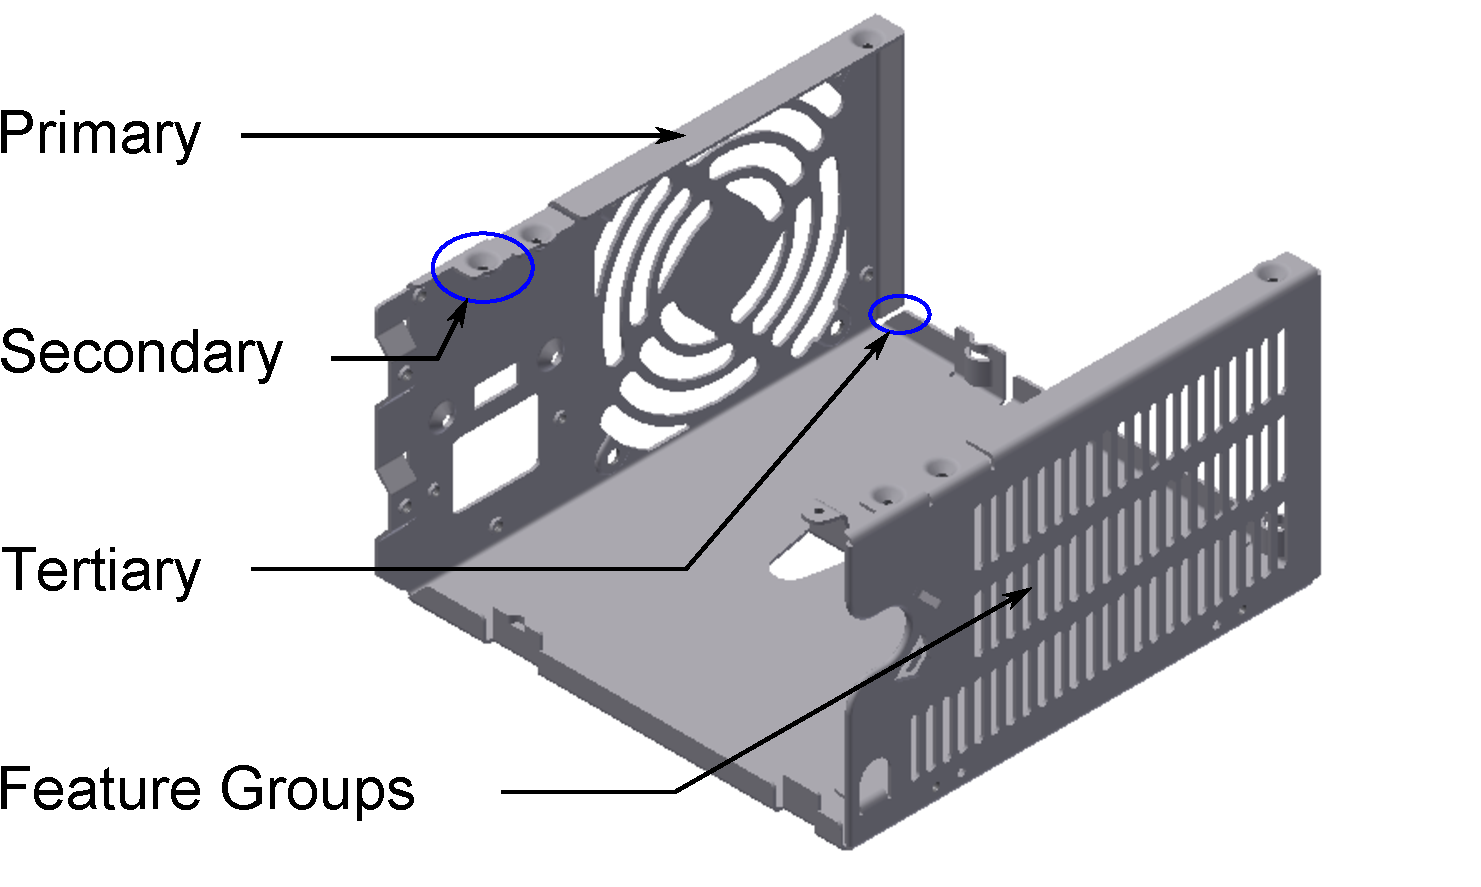
\includegraphics[width=0.62\linewidth]{images/SheetMetal_taxonomy_3.pdf}
		\caption{Sheet Metal Features Based on Proposed Taxonomy}
		\label{fig:defeaturing:classification}
	\end{figure}
	
%%\bigskip

Figure~\ref{fig:defeaturing:classification} shows example part with various sheet metal features classified as per the proposed taxonomy. %%Following section details out the defeaturing process using the same classification.

\todo{Review comments: Logic of dormant feature needs to be clearly explained (in the algorithm) Why it is appearing here? [IT HAS BEEN MOVED TO ITS OWN SECTION LATER]}

\todo{Review Comments: Explain these steps with figure. [DONE]. Give figures for what is resultant model after processing primary then model after processing secondary and then tertiary. [IMPLEMENTATION IS DONE IN A SINGLE LOOP. WILL NEED TO RE-FACTOR SO THAT SEPARATE OUTPUTS CAN BE COLLECTED. WILL TRY THIS LATER]}

\subsection{Defeaturing Algorithm Based on Sheet Metal Features \mbox{Taxonomy}} \label{sec:defeaturing:taxonomy}

This subsection details the steps used to identify the removable sheet metal features based on the taxonomy proposed in Section~\ref{sec:defeaturing:phase11}. 
\todo{Review comment: What is threshold? Who defines it, what is the typical value you have found after experimenting? [ADDED EXPLANATION]}
Threshold value is computed based on the experimentations done~\cite{YogeshCADandA2016} to assess the effect of different threshold values on the quality of resultant midsurface output. Parameter $D$, which is used as a size criteria for deciding irrelevance of a feature, is defined as threshold \%age ($p$) of the size of the CAD model. Size of the CAD model can be defined in multiple ways, such as, size of Bounding Box, volume, etc. Bounding box as a measure of size, is quick to compute but not accurate. Volume is more accurate than Bounding box but is compute intensive, especially for Brep based CAD model, where the model is composed of faces. Sum of areas of the faces is both, reasonably accurate and easier to compute the size. Thus the present research measures size of the model as sum of the areas of all the faces. The \%age value for threshold is typically based on expertize, application context and engineering judgment. Various experiments were conduced to correlate effect of \%age value of threshold on the gross shapes. Table \ref{tbl:litsurvey:defeatmids} summarizes the results and more details are presented in Appendix~\ref{appendix:threshold}. Based on those experiments typical threshold values used in the present research work are 5-10\%.

Defeaturing rules based on sheet metal features taxonomy are enumerated below:
\begin{enumerate}
[noitemsep,topsep=2pt,parsep=2pt,partopsep=2pt, leftmargin=*]
\item \textbf{Primary Features}: Not removed as these features mainly contribute to the gross shape. Examples are  Face-Wall, Flange, Bend, etc.
%	\begin{itemize} [noitemsep,topsep=2pt,parsep=2pt,partopsep=2pt]
%	\item Face-Wall
%	\item Flange
%	\item Bend
%	\end{itemize}
\item \textbf{Secondary Features}: Are removed based on the relative size with respect to the size of the whole model. Features smaller than the threshold are removed, whereas bigger ones are retained.
%	\begin{itemize} [noitemsep,topsep=2pt,parsep=2pt,partopsep=2pt]
%	\item Stamping
%	\item Cutout
%	\item Emboss 
%	\end{itemize}
	
\item \textbf{Tertiary Features}: Are removed irrespective of their size relative to the size of the whole model. 
%	\begin{itemize} [noitemsep,topsep=2pt,parsep=2pt,partopsep=2pt]
%	\item Lip
%	\item Rest 
%	\end{itemize}
	
%\item \textbf{Connecting Features}: These are not suppressed irrespective of their sizes, as removing them, will create gaps between the sub-shapes of the original part. Lacking these would create gaps, so these are retained irrespective of their relative size, small or large.
%Example is:
%	\begin{itemize} [noitemsep,topsep=2pt,parsep=2pt,partopsep=2pt]
%	\item Bend
%	\end{itemize}
		
\item \textbf{Feature Groups}: Are removed based on the collective relative size with respect to the size of the whole model. 
%\begin{itemize} [noitemsep,topsep=2pt,parsep=2pt,partopsep=2pt]
%	\item Mirror
%	\item Patterns
%	\end{itemize}
\end{enumerate}

 	\begin{figure} [!h]
		\centering
		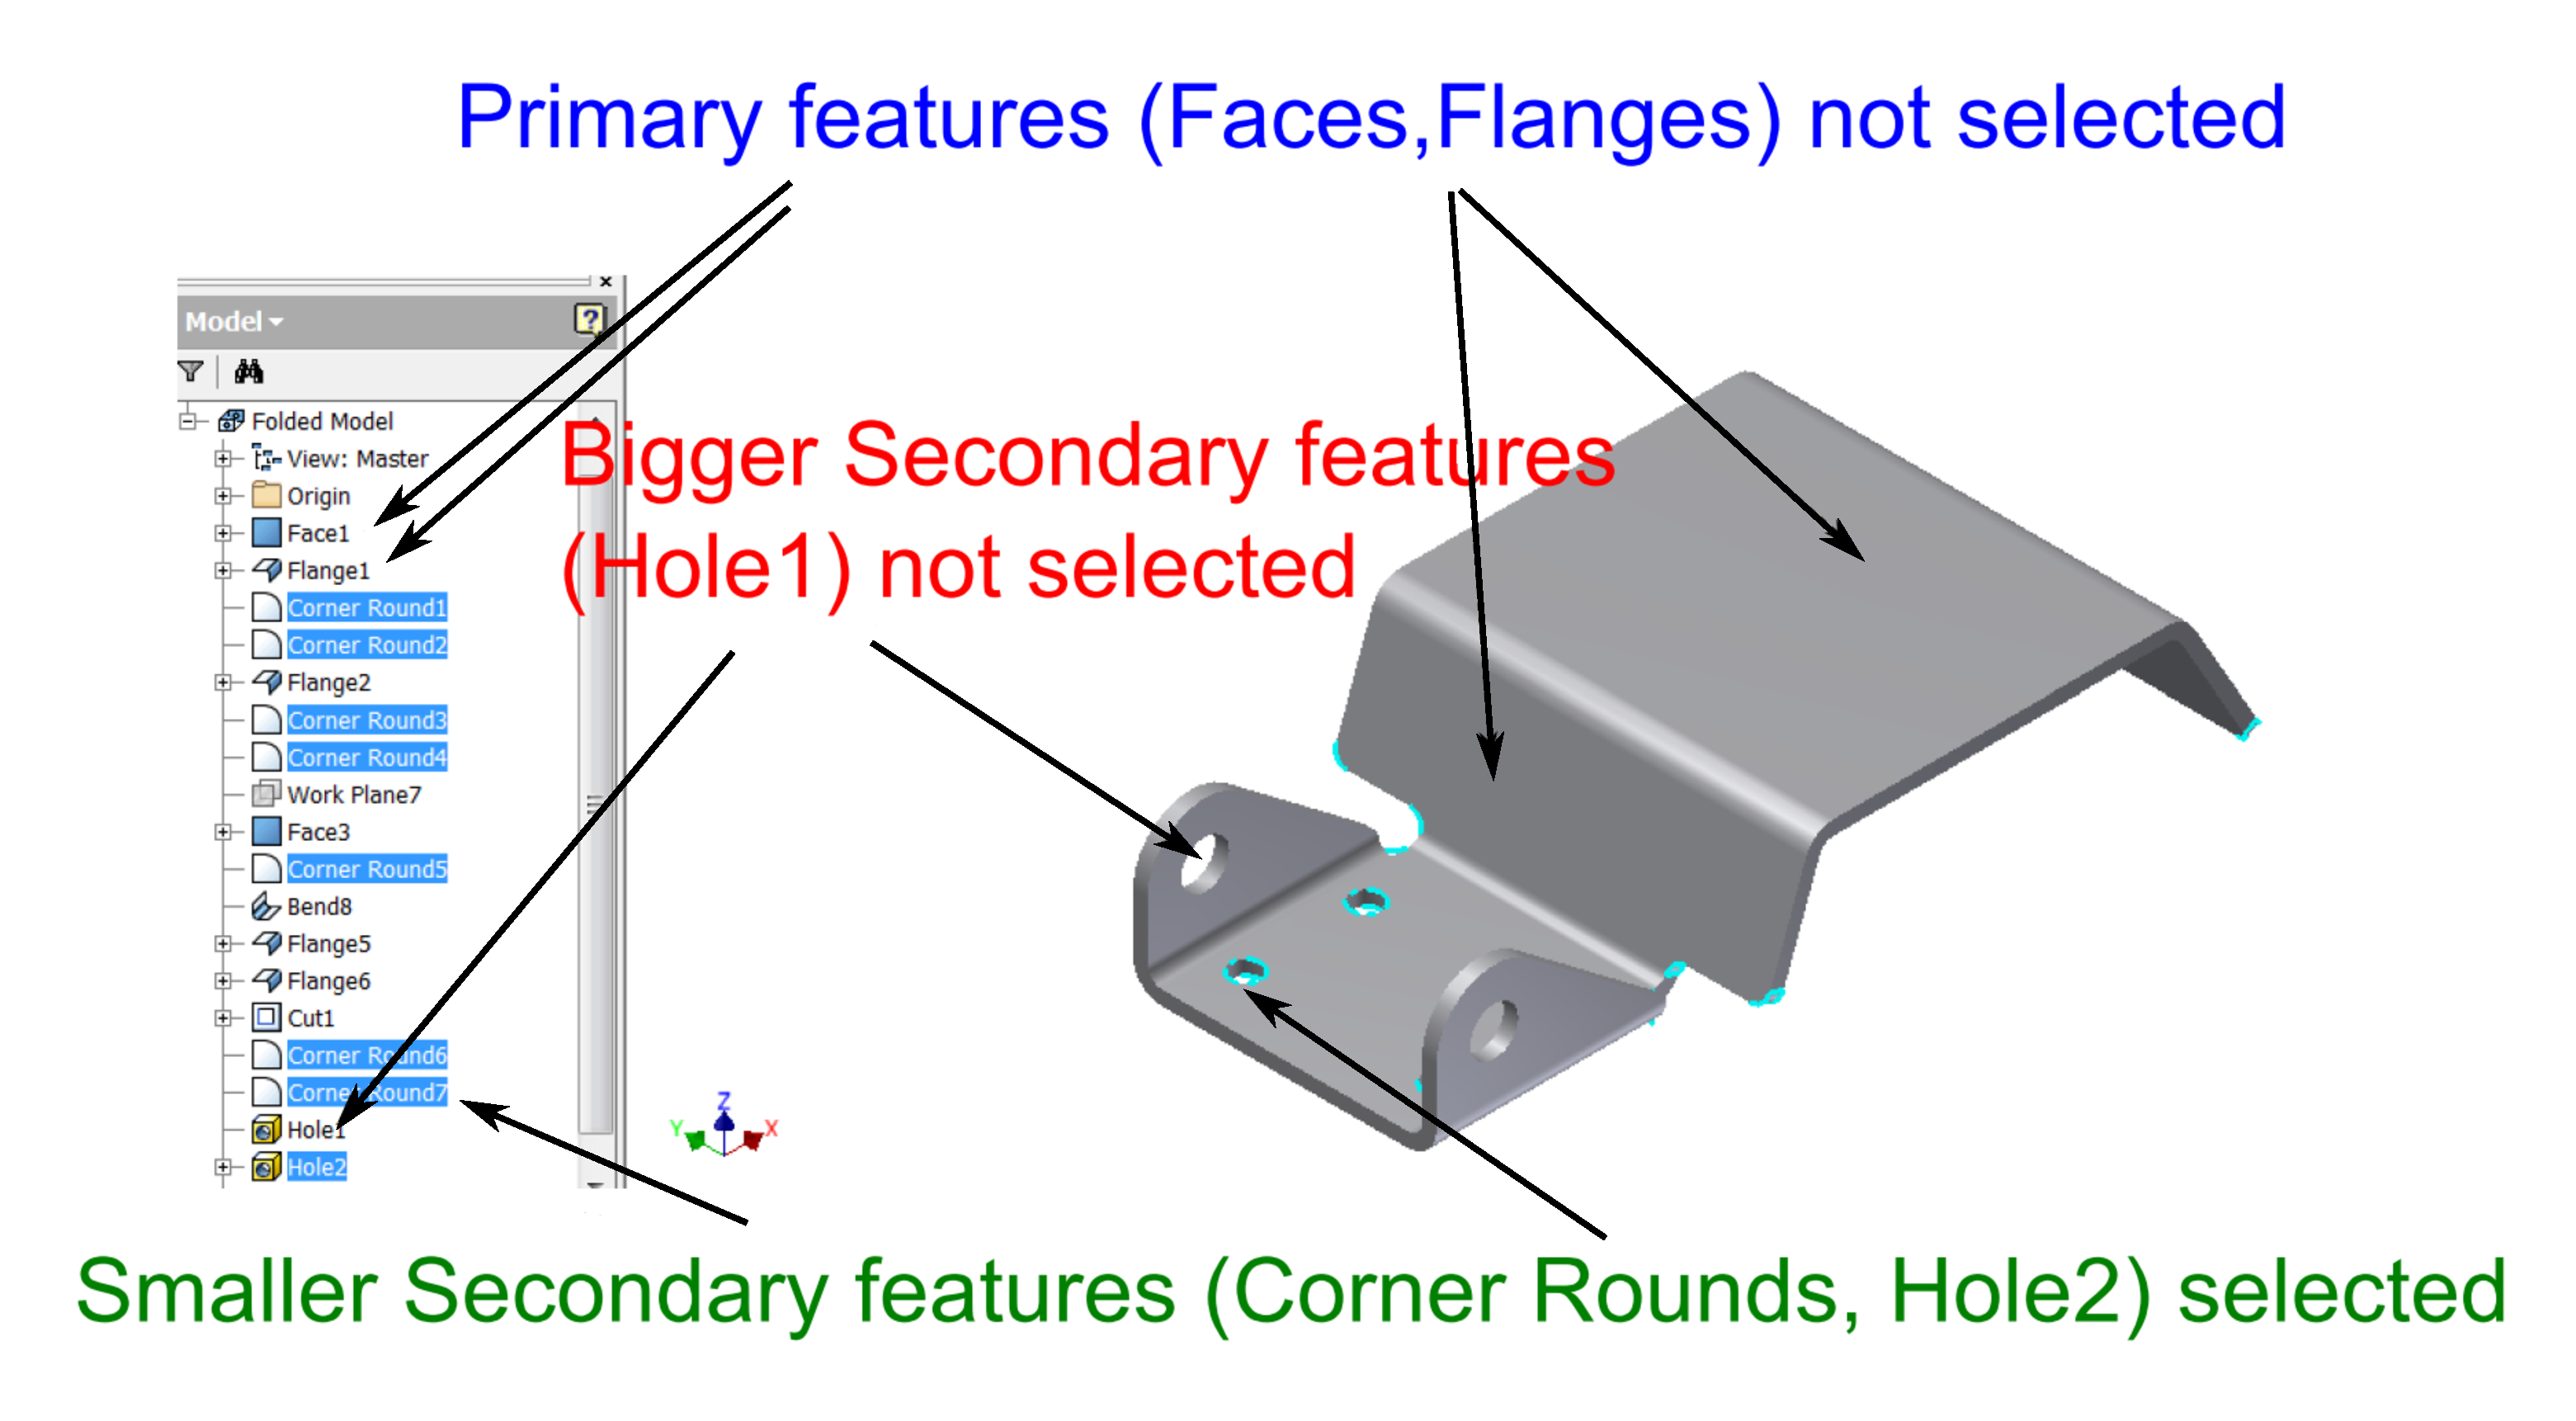
\includegraphics[width=0.62\linewidth]{images/SheetMetal_Ph1_Selection_Annotated_1.pdf}
		\caption{Defeaturing Based on Proposed Taxonomy }\label{fig:defeaturing:actions}
	\end{figure}
	
Figure~\ref{fig:defeaturing:actions} shows an example sheet metal part CAD model, with taxonomy based features categories shown, along with their defeaturing rules. Primary features such as Walls (Faces), Flanges are not removed. Secondary features whose face-size is less than the threshold are removed, but the larger ones are retained. With threshold as 5 \%, holes smaller than 5 \% of the model faces area, such as Hole2 and CornerRounds are selected but not the bigger holes such as Hole1.
 
%%\bigskip
 
%\subsubsection{Algorithm to identify candidate features for de-featuring based on Sheet Metal feature taxonomy:}
\begin{algorithm}[H]
	\caption{Phase I: Defeaturing Sheet Metal Features}
	\label{alg:defeaturing:phase1}
	\begin{algorithmic}[1]
		\REQUIRE A Sheet Metal FCAD model with access to the feature tree
		
%		\WHILE{$nextFace() != null$}
%			\STATE $F_i = currentFace()$
%			\STATE $Area_{face} \quad += F_i \rightarrow area()$
%		\ENDWHILE		
		\STATE $p = getPreDefinedThreshold()$
		\STATE $Area = sumAllFaceAreas()$
		\STATE $D = \frac{p}{100} \times Area$
		\WHILE{$f_i = currentFeature() != null$}
			\IF {$f_i \rightarrow isPrimaryFeature()$}
				\STATE continue
			\ELSIF {$f_i \rightarrow isTertiaryFeature()$}
				\STATE $sl \rightarrow add(f_i)$
			\ELSIF {$f_i \rightarrow isGroupFeature()$}
			  	\IF {$  f_i \rightarrow combinedArea() < D$}
			  		\STATE $sl \rightarrow add(f_i)$
				\ENDIF
			\ELSE
			  	\IF {$f_i \rightarrow area()  < D$}
			  		\STATE $sl \rightarrow add(f_i)$
%				\ELSIF  {$f_i \rightarrow isNegativeFeature()$}
%					\STATE $sl \rightarrow add(f_i)$ //Dormant feature
				\ENDIF				
			\ENDIF
		\ENDWHILE
		\STATE  $sl \rightarrow removeAll()$
		\STATE  $rebuildModel()$
	\end{algorithmic}
\end{algorithm}

%%\bigskip

Following are the steps taken for defeaturing CAD model based on sheet metal features taxonomy. Algorithm~\ref{alg:defeaturing:phase1} presents the same in pseudo-code form.

\begin{enumerate}
[noitemsep,topsep=2pt,parsep=2pt,partopsep=2pt]
\item The threshold \%age value is chosen. The threshold size is the threshold percentage times of the size of the model. The size of the model  is computed as the total of areas of all faces of the model. It is denoted as ``face-size'' of the model. Similarly, size of the feature is denoted as ``face-size of the feature'' and is the sum of area of the faces of the particular feature (Algorithm~\ref{alg:defeaturing:phase1}: lines 1-3).
\item The model feature tree is traversed and the current feature is applied with the defeaturing rules based on the newly proposed taxonomy (Figure~\ref{fig:defeaturing:tax_sm}, Figure~\ref{fig:defeaturing:actions}) (Algorithm~\ref{alg:defeaturing:phase1}: loop 4 to 18). 
\item The Primary features are not selected for removal so get skipped and do not get added to the removable-features list  (Algorithm~\ref{alg:defeaturing:phase1}: lines 5-6).
%\item The features are selected for removal based on the rules  as detailed out in section~\ref{sec:defeaturing:phase11} based on the newly proposed taxonomy (Figure~\ref{fig:defeaturing:tax_sm}). 
\item If the current feature is a ``Tertiary'' feature, then it is added directly to the removable-features list (Algorithm~\ref{alg:defeaturing:phase1}: lines 7-8).
\item If the current feature is a ``Group'' feature, then it's total face-size of the constituent features is checked against the threshold and if it is less then it is added to the removable-features list (Algorithm~\ref{alg:defeaturing:phase1}: lines 9-12).
\item If the current feature is a ``Secondary'' feature, then it's face-size checked against the threshold and if it is less then the feature is added to the removable-features list  (Algorithm~\ref{alg:defeaturing:phase1}: lines 14-16). 

\item Once all the features in the model are traversed, the features in the removable-features list are removed and the model is regenerated (Algorithm~\ref{alg:defeaturing:phase1}: lines 19-20).
%\item The `candidates list' is presented to the user for verification and changes, if necessary. 
%\item Features in the `candidates list' are removed.
%\item The model is regenerated and Defeaturing Effectiveness is computed using Eqn.~\ref{eqn:defeaturing:effectiveness}
%%
%%\item A list  ({\bf $sl$}) initialized to which the suppressible features are added. 
%%\item The model feature tree is traversed and the candidate features for suppression are identified based on a set of heuristic criteria such as ``Primary features are not to be suppressed'', ``Secondary features, if small, are selected'' etc.  (Figure~\ref{fig:defeaturing:actions}).
%%\item The identified features are added to {\bf $sl$}.
%%\item If ``Dormant' processing option is selected, all the negative features, which otherwise would not have qualified for the suppression are selected for suppression and added to  {\bf $sl$} . The bodies associated with these features are computed and cached. These bodies are later used to pierce the resultant Midsurface (Section~\ref{sec:defeature:dormant})
%%\item The {\bf $sl$} is presented to the user for verification and changes, if necessary. 
%%\item Features in  {\bf $sl$} are suppressed.
%%\item The model is regenerated and Defeaturing Effectiveness is computed using Eqn.~\ref{eqn:defeaturing:effectiveness}
\end{enumerate}


%%%\bigskip

%\subsection{Observations}

\todo{Review comment: Instead of Observations section, continue the algorithm section elaborate it wrt example. [DONE]}

\todo{Review commment: Need to explain this figure. [DONE]}

\begin{minipage}[t]{\linewidth}
\begin{tabular}[!h]{@{} p{0.3\linewidth} | p{0.3\linewidth} | p{0.3\linewidth}@{}} \toprule

\textbf{Input to Phase I} & \textbf{Detected Features} & \textbf{Output of Phase I} \\ \midrule

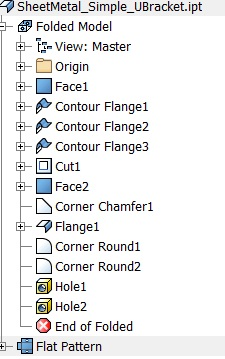
\includegraphics[width=0.92\linewidth]{images/DefeatPhase_I_t1} &
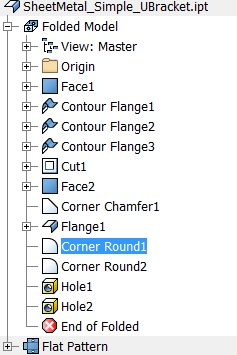
\includegraphics[width=0.98\linewidth]{images/DefeatPhase_I_t2} &
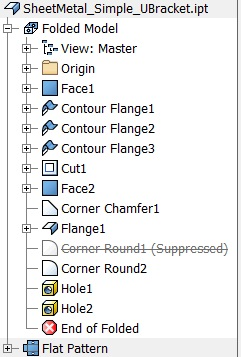
\includegraphics[width=0.99\linewidth]{images/DefeatPhase_I_t3} \\ \midrule

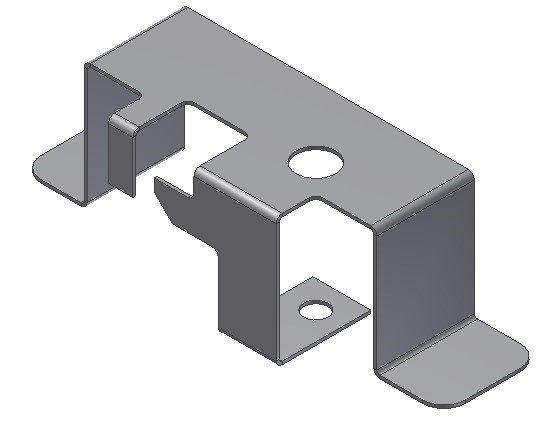
\includegraphics[width=0.98\linewidth]{images/DefeatPhase_I_1} &
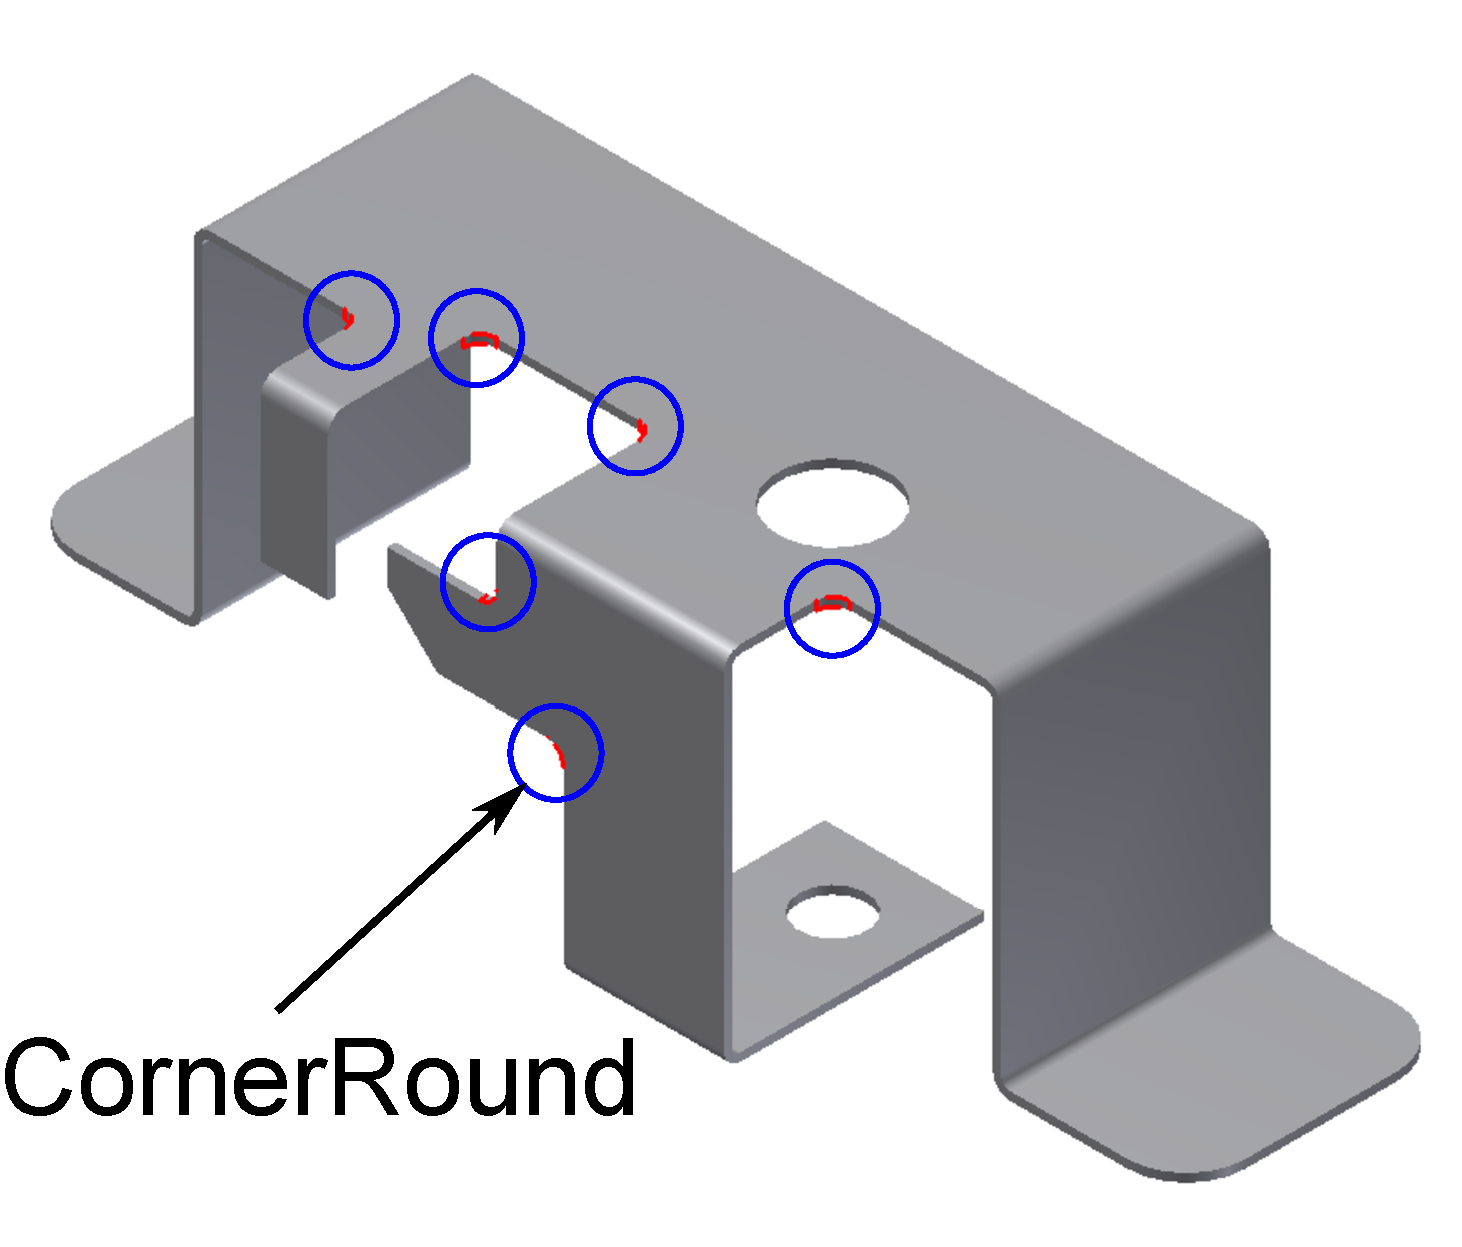
\includegraphics[width=0.98\linewidth]{images/DefeatPhase_I_2_new_nolables.pdf} &
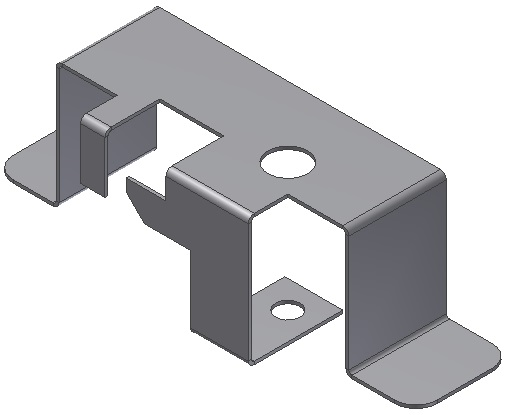
\includegraphics[width=0.98\linewidth]{images/DefeatPhase_I_3} \\ \bottomrule

\end{tabular}
\captionof{figure}{Phase I: Defeaturing Based on Feature Taxonomy and Size Threshold Approach}\label{fig:defeaturing:phaseI}
\end{minipage}

Figure~\ref{fig:defeaturing:phaseI} shows the process pictorially. The first column, called ``Input to Phase I'' shows input sheet metal features CAD model of a bracket part, along with its feature tree. The second column, called ``Detected Features'' shows the candidate features selected, such as `Corner Round1', on the model as well as in the feature tree, based on the steps mentioned above (also mentioned in Algorithm~\ref{alg:defeaturing:phase1}).  The third column shows the output of Phase I, showing the model with candidate features removed.

%%\bigskip




%%\bigskip

%\vspace{-3mm}

\todo{Review comment: At the end state what you conclude with this phase I processing. [DONE]}

With the Phase I over, sheet metal domain specific defeaturing is complete. This phase can be further enhanced by either customizing the threshold and/or by incorporating more features in the taxonomy based on further surveys and experimentations. It can be customized further, for different application domains, such as Injection Molding, by incorporating taxonomy specific to those domain. 

Following section details out the Phase II, i.e. defeaturing process based on geometric reasoning.

 %\vspace{-5mm}
 
\section{Defeaturing Based on Geometric Reasoning of CAD Model Features} \label{sec:defeaturing:phase2}

\todo{Review comment: Change title to Geometric reasoning of model features. [DONE. ADDED `CAD']}

The sheet metal feature based CAD models used in the present research work are built using `design-by-features' approach. At each feature step, the feature parameters first generate a feature primitive solid, known as ``tool-body''. Boolean operation is  performed between operands: the existing model at that stage and the tool body. During this operation, some portion of the tool-body-portion gets consumed within the existing model and the remaining portion of the tool body appears as a newly added feature in the CAD model. 


%%\bigskip

 	\begin{figure} [!h]
		\centering
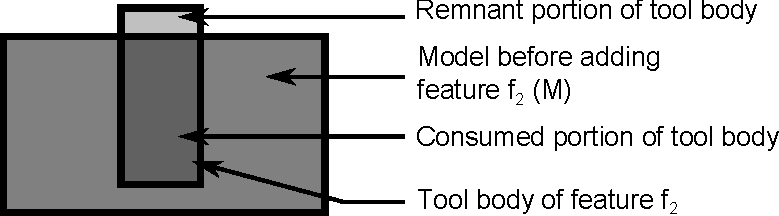
\includegraphics[width=0.62\linewidth,valign=t]{images/Solid_Simple_SmallProtrusion_labels_2.pdf}
		\caption{Remnant and Consumed Portions} \label{fig_remnant}
	\end{figure}
	
%%\bigskip

Figure ~\ref{fig_remnant} shows boolean operation between the existing CAD model denoted by  $M$ and the tool body of feature $f_2$. Some portion of the tool body gets consumed and is merged with the model whereas some portion remains outside. The portion remaining outside is referred as ``remnant feature'' portion. This phase involves the geometric reasoning to identify remnant feature portions on the input Brep CAD model.

Past attempts such as by Russ~\cite{Russ2012}, used full feature tool-body to determine the candidature for removal during defeaturing. This obviously gives incorrect results as the CAD model actually retains only the remnant portion of the feature. Size of only remnant portion should be considered for deciding the candidature for removal. Thus the present research  uses the size of the remnant portion for deciding removal of a feature and the algorithm to do this is presented below.


\subsection{Defeaturing Algorithm Based on Remnant Feature Portions}

%%In the feature based design paradigm, the CAD model is built step-by-step using features at each step.  At $j^{th}$ feature ($f_j$), the model built till then is referred as $M_{j-1}$.   Feature parameters are used to compute the ``canonical'' (tool-body) volume first, which is then booleaned to the model built till then. $V_j = volume (f_j)$. $V_j$ is the feature/canonical/tool-body volume of the feature $f_j$. $M_j = M_{j-1} \oplus V_j$. The model moves to the next state $M_j$ by boolean of existing state $M_{j-1}$ with the feature volume $f_j$ i.e. $V_j$.  During this operation, some portion of the canonical volume may get consumed, leaving behind the remaining (remnant) volume in the final solid  (Fig.~\ref{fig_remnant}). $V_j = R_{j} \cup C_j$. Some portion of $V_j$ gets consumed ($C_j$) and some remains ($R_j$). (Fig.~\ref{fig_remnant}). $M_j = M_{j-1} \cup  R_j$ and thus $R_j = M_{j} -   M_{j -1}$ is the remnant feature volume ~\cite{Lee2005}.

%%\begin{figure}[!htb]
%%\centering
%% 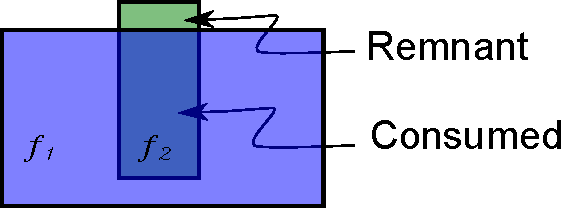
\includegraphics[width=0.35\linewidth]{images/Solid_Simple_SmallProtrusion.pdf} 
%% \caption{Remnant and Consumed portions of feature volume of  $f_2$}
%% \label{fig:defeaturing:remnant}
%%\end{figure}
%%  
%%Identification of suppressible features based on the feature volume computed from the full feature parameters yield incorrect results as the final shape may not retain the full feature volume. So, this work has devised a novel method  (Algorithm~\ref{alg:defeaturing:phase2}) to find the size of remnant feature volume to be used for deciding the suppressibility  (Fig.~\ref{fig:defeaturing:phaseII}) of the features. This phase starts with the final Brep for identifying the remnant portions of the features. This computation, being geometric in nature, can be generic to many applications, with an option to customize the threshold based on engineering judgment specific to the given application.
%%
%%\subsection{Approach}
%%
The input to this phase is the output CAD model from Phase I. In contrast to phase I, this phase does not involve traversal of the feature tree. Instead, it traverses faces of the final model i.e. the Brep model available at the end of the feature tree. As these faces have remained in the model till the end, they are termed as `remnant' faces. The Brep CAD solid model is termed as `final body'. Whenever a feature is added, it adds new faces to the existing Brep model. These new faces store information of the feature which created it, which is termed as the ``owner feature''. The owner feature information is stored on all faces of the Brep as attributes, typically referred as ``origination info''.

The intent of this phase is to group all the remnant faces belonging to a particular feature. This group is termed as `FaceGroup'. Then identify their respective feature owners, and decide their removability on the size of their remnant portions. The size of a FaceGroup can be calculated by various approaches like Influence Volume~\cite{SangHunLee2005} or the union of bounding-boxes, etc. The present work uses summation of the area of the remnant faces as the `Size' criterion and is called ``face-size''. The choice of area as the size criteria is based on ease of computability and reasonable accuracy to represent the remnant portion. 



Following steps present details of the algorithm used to identify remnant faces and thereby remnant features, to be removed based on the remnant portion of the tool body (Figure~\ref{fig_remnant}) (Algorithm~\ref{alg:defeaturing:phase2}).
\todo{Review comment: What is this (clusters table)? its unit, irs rationale, why you use this for what purpose, where are these in figure. [EXPLAINED HERE]}
\todo{Review comment: Give numbers to list items. [DONE]}
\todo{Review comment: A new term (FaceGroup) is coined here which is not explained here. [DONE]}

\begin{enumerate}
[noitemsep,topsep=2pt,parsep=2pt,partopsep=2pt]
\item Remnant faces of the final body are traversed. (Algorithm~\ref{alg:defeaturing:phase2}: loop 1 to 15).  
\item For each remnant face, its owner feature is retrieved (Algorithm~\ref{alg:defeaturing:phase2}: line 2).
\item Existing FaceGroups are searched for matching owner feature.
\item If a match exists, the face is added to that FaceGroup  (Algorithm~\ref{alg:defeaturing:phase2}: lines 4-8).
\item If a match is not found, then a new FaceGroup is created, the remnant face is added to it, it owner feature is set as the owner of the FaceGroup and this new FaceGroup gets appended to the list of FaceGroups  (Algorithm~\ref{alg:defeaturing:phase2}: lines 9-13).

\bigskip

\begin{minipage}{\linewidth}

\begin{minipage}[c]{0.48\linewidth}
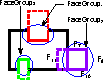
\includegraphics[width=0.8\linewidth,valign=t]{images/facegroups_1.pdf}
\captionof{figure}{FaceGroups} \label{fig_clusters}
\end{minipage}
%%\begin{figure}[!h]%[!h]
%%\centering     
%%\subfloat[Remnant and Consumed portions of $f_2$]{\label{fig_remnant}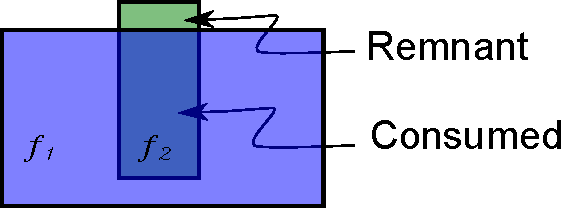
\includegraphics[width=0.5\linewidth,valign=t]{images/Solid_Simple_SmallProtrusion.pdf}} \quad
%%\subfloat[Formation of clusters]{\label{fig_clusters}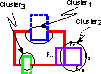
\includegraphics[width=0.25\linewidth,valign=t]{images/clusters.pdf}}
%%\caption{Phase II: Remnant feature definition, Cluster approach} 
%%\label{fig:defeaturing:phaseII}
%%\end{figure}
\hfill
\begin{minipage}[c]{0.48\linewidth}
\captionof{table}{FaceGroups Details}
\label{tbl_clusters}
\begin{tabular}[h]{@{} p{0.3\linewidth} p{0.25\linewidth} p{0.25\linewidth}@{}} \toprule
\textbf{FaceGroup Id} & \textbf{Face-size ($mm^2$)}& \textbf{Owner Feature}\\ \midrule
FaceGroup$_1$ & 0.25 	&  Extrude$_2$\\
FaceGroup$_2$ & 0.25  & Extrude$_3$\\
FaceGroup$_3$ & 0.125 & Hole$_1$\\ \bottomrule
%$f_{10}, f_{12}, f_{15}, f_{14}$ 	& Cluster$_4$\\ \bottomrule
\end{tabular}
\end{minipage}
\end{minipage}
%%\bigskip

%%\bigskip

Figure~\ref{fig_clusters} shows a schematic of existing Brep CAD model with 3 features booleaned to it. Thick lines are used to represent the remnant faces whereas dotted lines are used to represent the consumed faces. FaceGroup1 and FaceGroup3 are depression features, i.e. negative features, whereas FaceGroup2 is a protrusion feature i.e. a positive feature. In FaceGroup2, $F_{11}$ is a consumed face whereas Faces $F_{10},F_8,F_7$ are the remnant faces. So, FaceGroup2 represents remnant portion of the owner feature Extrude$_3$.

%\item  FaceGroups are formed with same owning features as shown in Figure~\ref{fig_clusters}, where the dotted portions show the consumed feature portions and the circles show the remnant portions. 
\item Face-sizes of the FaceGroups are computed. Table~\ref{tbl_clusters} shows face-size (in $mm^2$) along with owner feature of each FaceGroup.
\item A FaceGroup is removed if its face-size is below the threshold value (Algorithm~\ref{alg:defeaturing:phase2}: lines 16-18). The threshold used is same as the one used in Algorithm~\ref{alg:defeaturing:phase1}: lines1-3.
%%\item The candidates list is presented to the user for verification and changes, if necessary. 
\item Once all the FaceGroups are assessed, removable-features are removed from the feature tree and the model is rebuilt (Algorithm~\ref{alg:defeaturing:phase1}: lines 20-21).
%%\item The model is regenerated and Defeaturing Effectiveness is computed using Eqn.~\ref{eqn:defeaturing:effectiveness}
\end{enumerate} 

\bigskip

\begin{algorithm}[H]
	\caption{Remnant Feature Method}
	\label{alg:defeaturing:phase2}
	\begin{algorithmic}[1]
		\REQUIRE A CAD model with access to the feature tree. 
		\WHILE{$F_i = currentFace() != null$}  
			\STATE $feat = F_i \rightarrow owingFeature()$
			\STATE $addedFlag = false$
			\WHILE {$cl_j = currentFaceGroup() != null$}
				\IF {$cl_j \rightarrow owingFeature() == feat$}
					\STATE  $cl_j \rightarrow add(F_i)$, $addedFlag = true$
				\ENDIF
			\ENDWHILE
			\IF {$addedFlag == false$}
				\STATE  $cl_n = newFaceGroup()$
				\STATE  $cl_n \rightarrow owingFeature() = feat$
				\STATE  $cl_n \rightarrow add(f_i)$
			\ENDIF
		\ENDWHILE
		\WHILE {$cl_k = currentFaceGroup() != null$}
			\IF {$cl_k \rightarrow calculateSize() < D$} %\hspace{40mm} // Threshold D defined in Alg~\ref{alg1}
				\STATE   $sl \rightarrow add(cl_k)$
			\ENDIF			
		\ENDWHILE
		\STATE  $sl \rightarrow removeAll()$
		\STATE  $rebuildModel()$
	\end{algorithmic}
\end{algorithm}


\bigskip

Figure~\ref{fig:defeaturing:phaseII} shows the process pictorially. The first column, called ``Input to Phase II'' shows the sheet metal features CAD model of a bracket part partially defeatured in the Phase I,  along with its feature tree. The second column, called ``Detected Features'' shows the candidate features selected, such as Holes, on the model as well as in the feature tree, based on Algorithm~\ref{alg:defeaturing:phase2}. The Hole is made by cutting a cylinder like tool body. This tool body's dimensions are big enough to disqualify it from removal. But the remnant faces in the model are small enough to qualify this feature for removal. Third column shows the output of Phase II, showing the model with candidate features removed.
%\subsection{Observations}

\bigskip

\begin{minipage}[t]{\linewidth}
\begin{tabular}[h]{@{} p{0.3\linewidth} | p{0.3\linewidth} |  p{0.3\linewidth}@{}} \toprule

\textbf{Input to Phase II} & \textbf{Detected Features} & \textbf{Output of Phase II} \\ \midrule

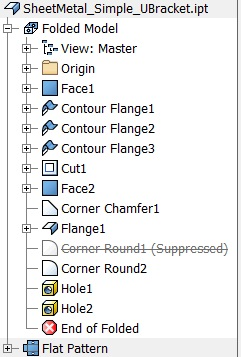
\includegraphics[width=0.92\linewidth]{images/DefeatPhase_II_t1} &
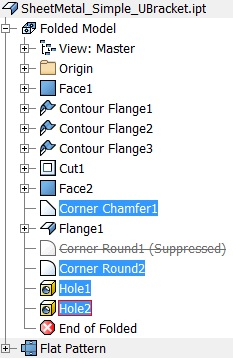
\includegraphics[width=0.98\linewidth]{images/DefeatPhase_II_t2} &
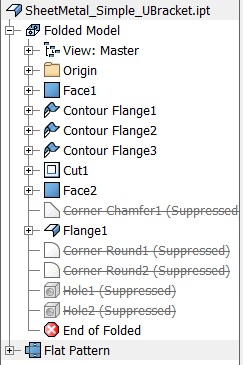
\includegraphics[width=0.99\linewidth]{images/DefeatPhase_II_t3} \\ \midrule

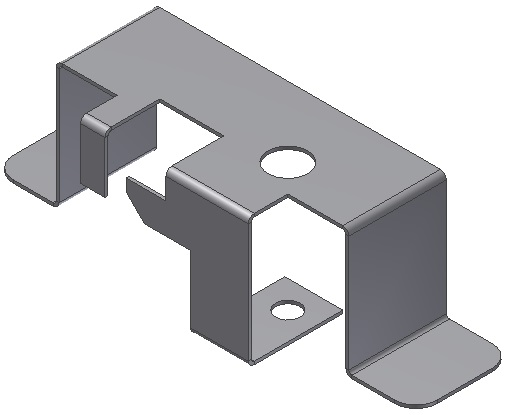
\includegraphics[width=0.98\linewidth]{images/DefeatPhase_I_3} &
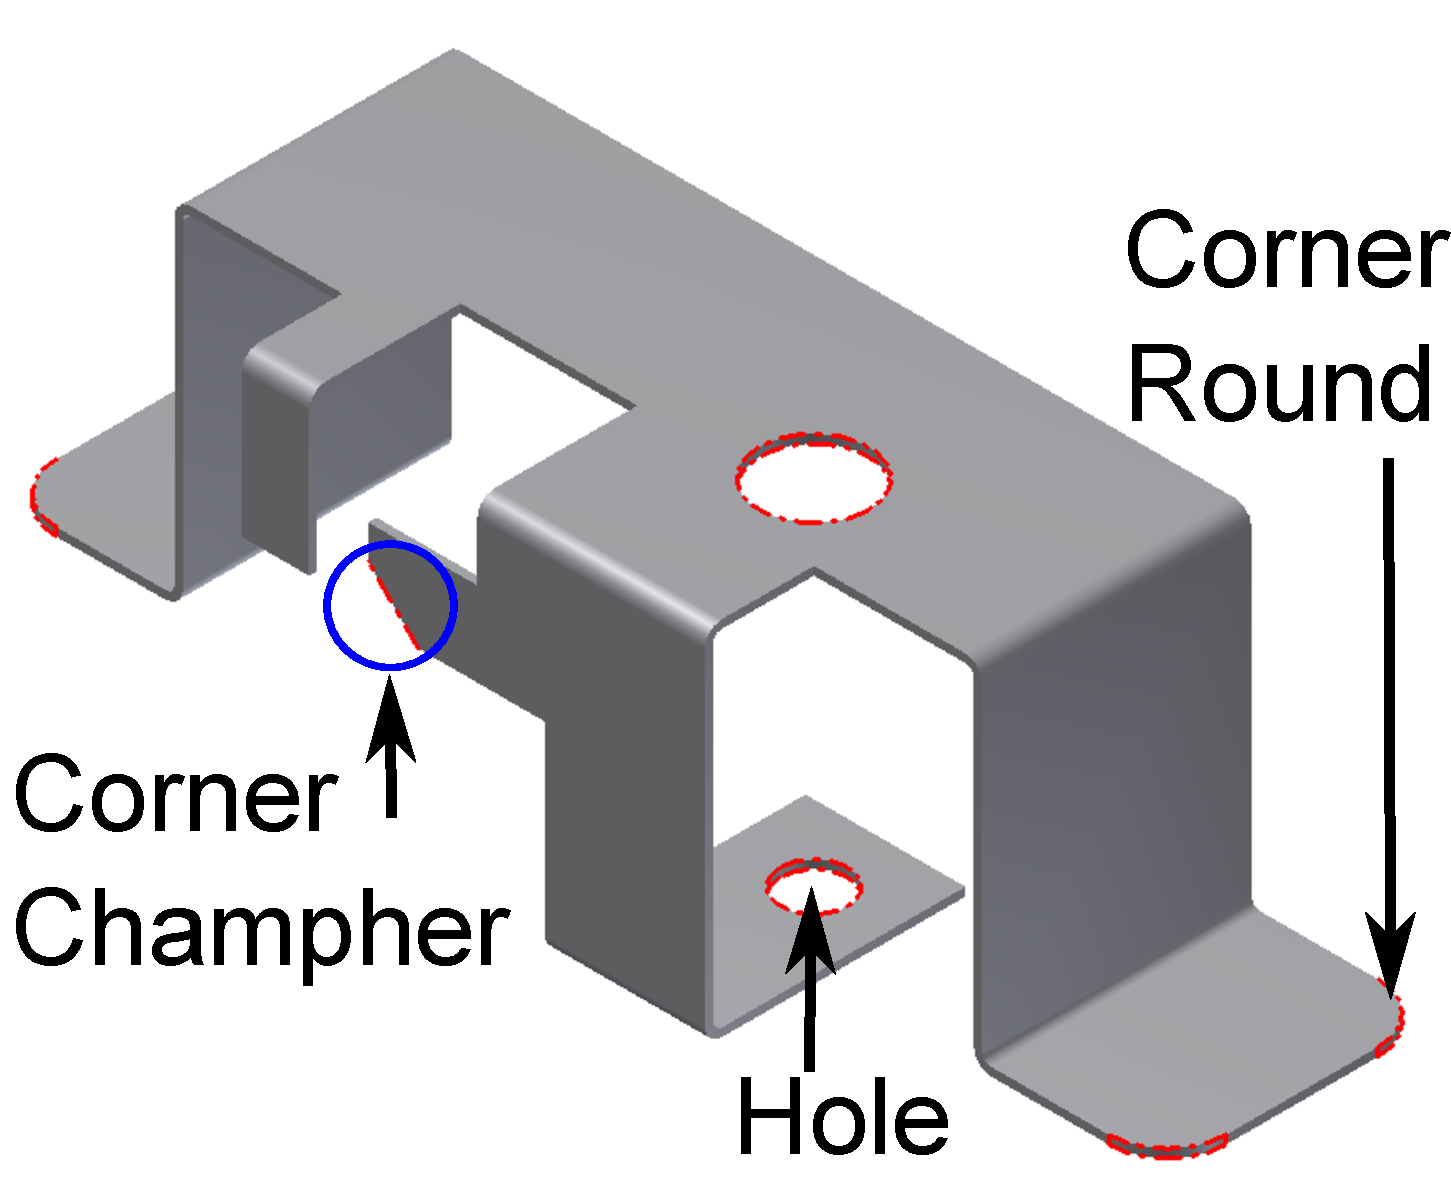
\includegraphics[width=0.92\linewidth]{images/DefeatPhase_II_2_new_wlables.pdf} &
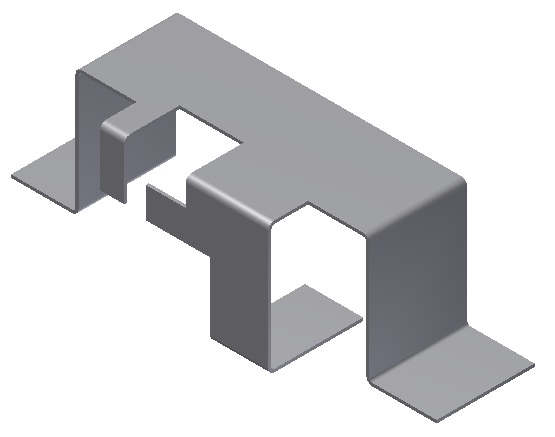
\includegraphics[width=0.98\linewidth]{images/DefeatPhase_II_3} \\ \bottomrule

\end{tabular}
\captionof{figure}{Phase II: Defeaturing Based on Remnant Feature Approach}\label{fig:defeaturing:phaseII}
\end{minipage}

\todo{Review comments: Drop this (observations) section. Continue previous section with elaborate explanation wrt figure. [DONE. ALSO: NEED TO IMPROVE FIGURE AND COMMENTARY. CURRENTLY FUZZY]}






\todo{Review comments: change column names. [THINKING OF ALTERNATIVES]}

%%\bigskip



%%\bigskip

After the first two phases, the given example of bracket model shows 50\% reduction in the number of features and 17\% reduction in the number of faces, at 5\% threshold value. The resulting gross shape has retained all important features necessary for the computation of a quality midsurface.

\section{Defeaturing Based on Dormant Feature Tool-bodies}\label{sec:defeature:dormant}

\todo{Review comment; Change title to bulk features. [NOT CHANGING THE TITLE AS OF NOW TO `DEFEATURING BASED ON BULK FEATURE REMOVAL' AS I AM NOT GETTING ITS MEANING. IN THE PARA, I AM TREATING `BULK' AS `LARGE'.]}

Bulk negative features, such as large Holes, Cutouts can be potentially problematic in further processes used in the midsurface computation, such as feature generalization (Chapter~\ref{ch:Abstraction}) and cellular decomposition (Chapter~\ref{ch:Midsurface}). But they can not be removed because they are necessary constituent of the gross shape. 

\todo{Review comment: First provide rationale as to why some features rather bulk in size need to be mad dormant rather than defeatured. [DONE]}

The results shown in Table~\ref{tbl:litsurvey:defeatmids} demonstrate that removal of negative features, even though they are relevant, can help computation of midsurface. But the drawback is, these features, being relevant would be missing on the midsurface. The present research work proposes to gain the computational advantage but at the same time does not want to loose the relevant features. This proposed approach is called as the Dormant Features approach. In this approach, relevant negative features are removed temporarily, but while doing so their feature bodies (called ``tool-bodies'') are preserved for later usage. After computing midsurface from such highly defeatured model, the preserved tool bodies are brought back and are re-applied on the midsurface. Thus, effect of those important, relevant negative features on midsurface is not lost. However temporary removal does substantially simplify the model which make midsurface computation quite convenient. Following section elaborates Phase III, the dormant features approach.


%\subsection{Approach}\label{sec:defeature:dormantapproach}
\subsection{Defeaturing Algorithm Based on Dormant Features}\label{sec:defeature:dormantalgo}

\todo{Review comment: What is the strategy to identity such features?. [ADDED]}

At this stage, Phases I and II are already over. All the small, irrelevant features are already removed. All the remaining features now, are the relevant features. These can include the negative features as well. In the steps mentioned below, in-spite of being relevant, the large negative features are temporarily removed, after storing their tool bodies. These bodies are kept dormant to be used later for piercing on the midsurface. Algorithm~\ref{alg:defeaturing:phase3} presents pseudo code of the approach and has been listed below: 

\bigskip


\begin{algorithm}[H]
	\caption{Phase III: Dormant Features Identification}
	\label{alg:defeaturing:phase3}
	\begin{algorithmic}[1]
		\REQUIRE A Sheet Metal FCAD model with access to the feature tree
		
%		\WHILE{$nextFace() != null$}
%			\STATE $F_i = currentFace()$
%			\STATE $Area_{face} \quad += F_i \rightarrow area()$
%		\ENDWHILE		
		\WHILE{$f_i = currentFeature() != null$}
			\IF {$f_i \rightarrow isNegativeFeature()$}
				\STATE $b_i = computeToolBody(f_i)$
				\STATE $bl \rightarrow add(b_i)$
				\STATE $sl \rightarrow add(f_i)$
			\ENDIF
		\ENDWHILE
		\STATE  $sl \rightarrow removeAll()$
		\STATE  $rebuildModel()$
	\end{algorithmic}
\end{algorithm}

\bigskip

\todo{Review comment: You are not giving any sense of being dormant here. [ADDED, BOTH, HERE AND IN ALGO]}

\begin{enumerate}
[noitemsep,topsep=2pt,parsep=2pt,partopsep=2pt]
\item The input CAD model feature tree is traversed (Algorithm~\ref{alg:defeaturing:phase3}: loop 1 to 7). 
\item  The current feature is tested if it is a negative feature, like Hole, Cutout, Extrude with subtractive boolean, etc. (Algorithm~\ref{alg:defeaturing:phase3} line: 2). 
\item The tool body is computed using its feature parameters (Algorithm~\ref{alg:defeaturing:phase3} line: 3). 
\item The tool-body is stored in a list (Algorithm~\ref{alg:defeaturing:phase3} line: 4). 
\item The current feature is added to list for removal (Algorithm~\ref{alg:defeaturing:phase3} line: 5). 
\item Once all the features in the feature tree are traversed, the features from candidate features list are removed and the CAD model is rebuilt (Algorithm~\ref{alg:defeaturing:phase3}: lines 8-9).
\end{enumerate}

%By the deferment of processing dormant features, generating midsurface patches gets simplified as these features are not present during their computation.  
\todo{Review comment: Clearly explain algorithm with figure. [IT SHOWS THE APPLICATION OF DORMANT AND NOT SELECTION. AM NEED TO REPLACE WITH A BETTER FIGURE, IF POSSIBLE]}


%%\bigskip




%%\bigskip
	
%\subsection{Observations}\label{sec:defeature:dormantobs}

%%%%\bigskip
%%
%% 	\begin{figure} [!h]
%%		\centering
%%\includegraphics[width=0.45\linewidth,valign=t]{images/dormant_labels.pdf}
%%		\caption{Re-application of the Dormant Feature Tool-body on Midsurface} \label{fig_dormant}
%%	\end{figure}
%%	
%%%%\bigskip

	\begin{figure}[h!]
	\centering 
	%\includegraphics[width=0.85\linewidth]{images/facepairing}
	\subfloat[Input CAD Model]{\label{fig:midsurfcelljoin:beforedomant}\includegraphics[width=0.5\linewidth,valign=t]{images/UBracket_part}} \hfill
	\subfloat[Semi-Final Midsurface]{\label{fig:midsurfcelljoin:semimids}\includegraphics[width=0.49\linewidth,valign=t]{images/MidsurfBracket}} \hfill
	\subfloat[Dormant Tool Bodies Re-application]{\label{fig:midsurfcelljoin:dormant}\includegraphics[width=0.49\linewidth,valign=t]{images/MidsurfDormantBodies_2}} \hfill
	\subfloat[Final Midsurface]{\label{fig:midsurfcelljoin:finalmids}\includegraphics[width=0.49\linewidth,valign=t]{images/MidsurfAfterDormant}}
	\caption{Re-application of the Dormant Feature Tool-bodies on Midsurface}
	\label{fig_dormant}
	\end{figure}
	
Figure~\ref{fig_dormant} shows reapplication i.e piercing of the dormant feature tool bodies. Figure~\ref{fig:midsurfcelljoin:beforedomant} depicts model before detection of the dormant features. Figure~\ref{fig:midsurfcelljoin:semimids} shows midsurface computed after removal of the dormant features. The cached dormant feature tool bodies are brought back and are re-applied on the midsurface, as shown in Figure~\ref{fig:midsurfcelljoin:dormant}. So, the presence of relevant negative features is made sure in the final midsurface as depicted in Figure~\ref{fig:midsurfcelljoin:finalmids}. Thus ensuring faithful representation of all the prominent features on the midsurface. 
%
%\begin{minipage}{0.95\textwidth}
%\begin{minipage}[c]{0.42\linewidth}
%\includegraphics[width=0.75\linewidth,valign=t]{images/dormant}
%\captionof{figure}{Re-application of the Dormant Feature Tool-body on Midsurface} \label{fig_dormant}
%\end{minipage}
%\hfill
%\begin{minipage}[c]{0.56\linewidth}
%% (Refer example in Section~\ref{sec:results:computation} for more details).
%Stored dormant features' tool bodies are reapplied on the midsurface. More details at Figure~\ref{fig:midsurfcelljoin:midsdorm}.
%\end{minipage}
%
%\end{minipage}

\todo{Review comment: Provide  a paragraph of your comment on what is outcome of these three phases. [DONE]}

Table \ref{tbl:defeaturing:benchmarking} shows a brief comparison of the present research work, as implemented in \mysystemname, with the other defeaturing approaches, such as, by Brian Russ~\cite{Russ2012},  Sungchan Kim et. al~\cite{Kim2005} and Sang Hun Lee~\cite{Lee2005}.

\bigskip
%------------------------------------------------------------------------------------
\begin{minipage}[t]{0.9\linewidth}
  \centering
   \captionof{table}{Comparison of the Present Research with Other Methods}
  \label{tbl:defeaturing:benchmarking}
%  \resizebox{\linewidth}{!}{ 
\begin{longtable}[htp]{@{} p{0.16\linewidth} |p{0.18\linewidth} | p{0.18\linewidth}| p{0.18\linewidth} |p{0.18\linewidth}@{}}
\toprule
\textbf{Methods} & \textbf{Russ~\cite{Russ2012}} &	\textbf{Kim~\cite{Kim2005}} &	\textbf{Lee~\cite{Lee2005}} & \textbf{\mysystemname}\\
\midrule
\textbf{Input} & Features	& Brep	& Features	& Features\\
\midrule
\textbf{Approach} & Suppresses if feature size is less than threshold.&
Wrap-around. Negative volumes removed totally. &
Feature volumes are reordered in sorted manner.&
Suppress based on taxonomy and remnant volumes.\\
\midrule
\textbf{Advantages} & Automatic identification of non-critical features &
 Does not need features; Works on Brep&
 Multiple defeaturing levels possible& More accurate criteria for defeaturing
\\
\midrule
\textbf{Limitations} & Limited to FEM as BC and Load path features are not suppressed. &
Concave edge filling creates odd shapes. Principal shape is lost. &
Due merged Cellular model, update capability is lost forever. &
Taxonomy needs to be updated for new features\\	
\bottomrule
\end{longtable}
%}

\end{minipage}


\bigskip

\added{The comparison indicates that the defeaturing approach presented in this chapter significantly reduces the number of faces in the CAD model thus simplifying it considerably for the purpose of midsurface computation. It, however, still ensures that the gross shape of the input CAD model is retained so that underlying design intent is not lost.}

In summary, Phase I removes features from the input CAD model based on the newly proposed sheet metal features taxonomy. The model gets further simplified in Phase II using remnant feature portions approach. Phase III simplifies the model further by completely removing all the negative features. After completion of all three phases of defeaturing the input sheet metal features CAD model is more or less reduced to its gross shape. This is optimum and effective level of defeaturing. Any further removal of the features will disturb the original gross shape intent.

Following section presents a newly proposed measure to assess the effectiveness of the defeaturing process.

\section{Effectiveness of Defeaturing}\label{sec:defeaturing:effectiveness}

\todo{Review comment: Not clear whether these are existing approaches. [THESE ARE EXISTING APPROACHES]}

Effectiveness of the defeaturing process is computed using a wide variety of methods\added{, such as quantitative reduction, MAT, Mesh based, etc.} They can be classified into input-based and output-based methods. In the input-based method, engineering judgment is used to set the initial defeaturing parameters, such as, size threshold, feature taxonomy, etc. and the output resulted is considered as the valid~\cite{MobleyCarrollCanann1998}. In the output-based method, some initial defeaturing parameters are set and the output is assessed against predefined benchmarks, such as, reduction in volume or number of faces or features, etc. The process is repeated till the benchmarks are  achieved. 

In the present research, the input-based method is used to assess the effectiveness of defeaturing. It is computed by measuring {\bf Percentage reduction in the number of faces}. Measurements are done before and after a particular defeaturing phase. More the percentage, more effective is the defeaturing process. A measure of reduction in number of features can also be used in place of faces to form another criterion for assessing the effectiveness. The present research work collects following parameters to compute the effectiveness:

\todo{Review comments: Rename Phase I, II. [RETAINED THESE NAMES, AS THEIR MEANING IS EXPLAINED IN PARAGRAPH ABOVE]}

	\begin{enumerate}
	[noitemsep,topsep=2pt,parsep=2pt,partopsep=2pt]
%	\item Total area of the Faces ($aF$)  ($mm^2$) 
%	\item Threshold size is some (say, 5 percent) of $aF$ ($sP$ $mm^2$)
	\item Total number of the faces in the original part ($nF$)
%	\item Number of sheet metal features suppressed in Phase I ($nS$)
	%\item Time spent in detecting the suppressible features in Phase I ($tS$ sec) 
%	\item Number of faces remaining in the model after Phase I ($mF$)
%	\item Number of \deleted{generic} features suppressed in Phase II ($nR$)
	%\item Time spent in detecting the suppressible features in Phase II ($tR$ sec)	
	\item Number of faces remaining in the model after defeaturing ($rF$)
	\item Defeaturing effectiveness ($pR$) (\%)
	\begin{equation}\label{eqn:defeaturing:effectiveness}  pR = (1 - \frac{rF}{nF}) \times 100\end{equation}
	\end{enumerate}

Defeaturing effectiveness ($pR$) gives quick idea of the order of magnitude of defeaturing.

Following section demonstrates efficacy of the proposed defeaturing approach by evaluating it against CAD model of a real-life test part.

\todo{[REMOVED OTHER METHODS. NOT VERY CONVINCING]}

%%Apart from $pR$, there could be some other and more involved criteria that can be used as follows:
%%	\begin{itemize}
%%	[noitemsep,topsep=2pt,parsep=2pt,partopsep=2pt]
%%	\item \textbf{Medial Axis Comparisons}: Medial Axis Transform (MAT~\cite{Ramanathan2004}) is a skeletal representation of a model. Model, with lots of details will typically generate MAT with branches at the location of details, whereas a simplified model, i.e. without numerous detauils, will not have branches at those locations. Figure~\ref{fig_matbranch} shows how MAT of a simple shape and a shape with extra detail differs. So, Comparison of MAT in case of model before and after defeaturing, by comparing branches can give idea about the effectiveness of the defeaturing process.
%%	
%%%%\bigskip
%%
%% 	\begin{figure} [!h]
%%		\centering
%%\includegraphics[width=0.55\linewidth,valign=t]{images/matbranch}
%%		\caption{Introduction of a detail adds a branch in MAT (Source~\cite{Chen1998})} \label{fig_matbranch}
%%	\end{figure}
%%	
%%%%\bigskip	
%%	
%%\todo{[REMOVED MESH COMPARISON. NOT VERY CONVINCING]}	
%%%	\item \textbf{Mesh}: Comparing faceted mesh generated by body defeatured by {\bf Smarf} with the mesh simplified by any benchmark mesh simplification methods can give the effectiveness measure.
%%	\item \textbf{Size}: Comparison of volume of the original and the defeatured model.
%%	\item \textbf{Shape deviation}: Using Part-Compare functionality, maximum deviation between the original and the defeatured, can be calculated. This deviation should be within predefined limits.
%%\end{itemize}


